\documentclass[paper=A4, pagesize, parskip=full]{scrreprt}
\linespread {1.25}

\usepackage[T1]{fontenc}
\usepackage[utf8x]{inputenc}
\usepackage[english]{babel}
\usepackage{fixltx2e}

\usepackage[nonamebreak]{natbib}

% used colors see http://en.wikibooks.org/wiki/LaTeX/Colors for more
\usepackage[usenames,dvipsnames]{xcolor}

\usepackage{ae} % somehow beautifies the output, don't know why
\usepackage[usenames,dvipsnames]{xcolor}
\usepackage {ellipsis, ragged2e}
\usepackage[babel]{csquotes}
\usepackage{microtype}

\PassOptionsToPackage{hyphens}{url}
\usepackage[pdfborder={0 0 0}, breaklinks, pdftex]{hyperref}
\hypersetup{colorlinks, linkcolor={Blue}, citecolor={Blue}, urlcolor={Blue}}
\urlstyle{same}

\usepackage{longtable}
\usepackage{datatool} % to include table data from .csv
\usepackage{lscape} % to turn the tables


\usepackage{graphicx}
\usepackage{nameref} % gets the name of a chapter when refering to the label with \nameref{chapterName}

%\usepackage{minutes}

% package and styles for code listings
\usepackage{listings}
\usepackage{courier}
\lstset{
         basicstyle=\small\ttfamily, % Standardschrift
         numberstyle=\small,          % Stil der Zeilennummern
         numbersep=5pt,              % Abstand der Nummern zum Text
         tabsize=2,                  % Groesse von Tabs
         extendedchars=true,         %
         breaklines=true,       
         numbers=left,
	  numbersep=6pt,
         frame=blr,
  	   commentstyle=\itshape\color{ForestGreen},
        keywordstyle=\bfseries\color{Blue},
        stringstyle=\color{Mahogany},
         showspaces=false,           % Leerzeichen anzeigen ?
         showtabs=false,             % Tabs anzeigen ?
         xleftmargin=24pt,
         xrightmargin=19pt,
         framextopmargin=5pt,
         framexleftmargin=10pt,
         framexrightmargin=10pt,
         framexbottommargin=-5pt,
         framesep=14pt,
         captionpos=top,
	   belowcaptionskip=-1pt,
         showstringspaces=false,      % Leerzeichen in Strings anzeigen ?   
         language=bash,
         escapeinside={{?}{?}}     
}
\lstset{language=bash}
\lstset{morekeywords={git, clone, status, push, checkout, pull, merge, branch, add, commit }
}
\lstloadlanguages{PHP, HTML, bash, Ruby, C, C++, make}

\usepackage{caption}
\DeclareCaptionFont{white}{\color{white}}
\DeclareCaptionFormat{listing}{\colorbox{MidnightBlue}{\parbox{\textwidth}{\hspace{10pt}#1#2#3}}}
\captionsetup[lstlisting]{format=listing,labelfont=white,textfont=white, singlelinecheck=false, margin={0mm}}


%%%%%%%%%%%%%%%%%%%%
%
%  Put together the parts of the document
%
%%%%%%%%%%%%%%%%%%%%
\begin{document}
\bibliographystyle {natdin}

% include every item in the bibliogaphy, also not cited ones
\nocite{*}

\begin{titlepage}
\vspace*{2cm}

\begin{center}
\Huge
Unplagged Developers Manual\\
\large
\vspace{0.5cm}
\rule[3mm]{1cm}{0.05mm}\\
Building the Plagiarism Detection Cockpit\\
\normalsize
\vfill
Term paper for the master project I \\ Mentoring Teacher: Prof. Dr. Debora Weber-Wulff\\
\vfill

Department Economics II\\
HTW Berlin -- University of Applied Sciences\\

\rule{8.2cm}{0.2mm}\\
Elsa Mahari (s0534556) \href{mailto:elsa.mahari@gmx.de}{\textless Elsa.Mahari@gmx.de\textgreater}\\
Dominik Horb (s0534217) \href{mailto:horb@htw-berlin.de}{\textless horb@htw-berlin.de\textgreater}\\
Tien Nguyen (s0512510) \href{mailto:s0512510@htw-berlin.de}{\textless s0512510@htw-berlin.de\textgreater}\\
Benjamin Oertel (s0522720) \href{mailto:contact@benjaminoertel.com}{\textless contact@benjaminoertel.com\textgreater}\\
Heiko Stammel (s0534218) \href{mailto:heiko.stammel@googlemail.com}{\textless heiko.stammel@googlemail.com\textgreater}\\


\end{center}
\end{titlepage}

% arabic page numbering should start after introduction so we start with roman, but after the title
\pagenumbering{Roman}

% group with custom link color to make sure not every item in the toc is weirdly colored
\begingroup 
  \hypersetup{linkcolor=black}
  \tableofcontents
  \listoffigures
\endgroup

\chapter*{Introduction}\addcontentsline{toc}{chapter}{Introduction}

Nine month after the start of development, the time of the masters project Unplagged at the HTW has now come to an end for the 
initial team members. Hopefully though, 
this isn't the end of the lifecycle of the software Unplagged that was created during that stretch. Some of us will try to continue working on it afterwards and maybe we are even able to attract some other developers to help this open source project in the long run if we are lucky. It was a good experience after all and the foundation feels good and strong.

Although there are no direct connections, this present document is at least in some ways a sequel to the Developers Manual, that was
written after the first semester of this project. In some instances it assumes prior knowledge of things already described there, so that it doesn't unnecessarily need to be repeated here.
All in all, we are going to give a more technical insight into the system than in the report before, which concentrated mostly
on the project management and development environment aspects. We will also try to critically 
analyze the problems that were faced and the mistakes that were made over the course of those
two semesters.

For all the team members, the development of Unplagged up to this point was one of 
the biggest 
projects that we ever had to start and needed to bring to a state of usable 
maturity on our own. Most of us came across big or even huge projects at work some time, but the process until 
the first release was mostly long over and replaced by bugfixing and the eventual feature release.
So those team building phases forming, storming, norming and perfoming that Bruce Tuckman famously described\citep{tuckman1965},
were something we saw in this project for the first time in full scale.

During our time of study, it was also one of the first projects, 
where we couldn't really envision in the beginning, how the end result would need to look like. It surely happened before at some points, but the implications of wrong decisions in the beginning weren't nearly as big then, as with such a long running development process like here.

With other projects before, there were also often requirements similar to some
parts of software systems we already knew and just needed to adapt to the current purpose.
This mostly gave us some hints of the feasibility and the best approach to solve a problem.
With Unplagged this was somehow different.

First of all, the idea for the project came from outside the team with very short time to research before the team building what it would be 
about and second, we didn't have any experience with plagiarism research at all. 
This means that we couldn't even imagine how the necessary workflow would need to look like, so we started out with one abstract idea of the system 
from outside of the development team, turned that into a different idea for every team member and eventually had to break it down to one software system.

We discoverd some similarities to project managements systems like Redmine or Jira and maybe Google Docs after a while, but at the start this wasn't really obvious.

Luckily enough, the choices of technologies, architecture or programming languages we made in the beginning, didn't came to haunt us up to this point. Without the experiences we made at internships or work this probably would have been a different story though.

\section*{Chapter Overview}\addcontentsline{toc}{section}{Chapter Overview}

\begin{description}
\item[\ref{chap:Overview}. \nameref{chap:Overview}] \hfill \\
This first chapter will give a very brief overview of the preconditions and project structure, analyzing it by some key figures and setting those into relation to the project achievements so far. It will also describe the \enquote{toolbox} of
frameworks and libraries that were integrated to have at our disposal for the development.
\item[\ref{chap:Features}. \nameref{chap:Features}] \hfill \\
Here we will describe the features and workflow implemented in the system so far.
\item[\ref{chap:Showtime}. \nameref{chap:Showtime}] \hfill \\
The chapter \nameref{chap:Showtime} will explain the preparations that were made for the presentation of the project results at the showtime.
\item[\ref{chap:summaryAndOutlook}. \nameref{chap:summaryAndOutlook}] \hfill \\
In the last chapter the main points are the discussion of the mistakes and
problems that were made during the development, with a focus on possible provisions against recurrence in future projects and an
outlook on the future of Unplagged.
\end{description}

\section*{Conventions}\addcontentsline{toc}{section}{Conventions}

To markup important words in the text, the following typographical conventions are used:

\begin{description}
\item \textit{Italic} \hfill \\
  First used technical terms
\item \texttt{Constant Width} \hfill \\
  Programm code, file names, paths
\item \textbf{\texttt{Bold Constant Width}} \hfill \\
  Variables that have to be changed by the user
\end{description}

% to ensure that the arabic numbering starts after the preface
\pagenumbering{arabic}
\chapter{Project Overview}\label{chap:Overview}

The main project description we started to work with was quite short with about 300 words and was also hugely complemented and clarified in meetings with Prof. Weber-Wulff. Nonetheless it contains very important bits and pieces that are the foundation of what was built during the project:

\begin{quote}
\enquote{Right. I'm the plagiarism \enquote{huntress}. I've tested plagiarism detection software since 2004. Mostly, they suck. They either don't work, or are a pain to use, or both. I've spent 10 years trying to educate people about plagiarism, and still the media thinks I have a magic secret for discovering plagiarism, as demonstrated on the GuttenPlagWiki and the VroniPlagWiki. What actually happens there is that quite a number of tools are used for preparing texts, discovering possible sources, comparing them, and documenting them. The last part is done by hand and takes an enormous amount of time.

The idea is to set up a Plagiarism Detection Cockpit that integrates all sorts of bits and pieces, but leaves the teacher in command. It is not to be a general test system that spits out a number for every paper submitted, although the integration of as many such systems as possible will be one of the necessary features of the system. There will be a lot of thought needed for the interface design, as there are massive amounts of data that need to be displayed. How can this be compressed and fit on a screen? For example, a barcode-generation needs to be integrated.

The goal will be to provide a tool that easily produces simple-to-read documentation and deals with all sorts of nastiness that might turn up on the way. The tool must be multi-lingual and open source. It would also be cool to integrate some of the little tools such as the Android-based OCR-Scanner that was developed in the SS 2011. I would like for the team to use an agile development methodology so that we can continuiously test with teachers and professors and *Plaggers.

One of the first tasks will be collecting up the computing literature on the topic of plagiarism discovery. A wiki needs to be set up with links to material (online and offline), comments on the papers, and as many navigational indices as possible.}\citep{projectDescription}
\end{quote}



\chapter{Features}\label{chap:features}

\section{Notifications and Comments}

The following section describes an important part of the application, especially for registered users: the notification system and the opportunity of adding comments basically to any resource in the system.

\subsection{Activity stream}
It displays the most recent events in the portal in descending order. Each activity (see figure \ref{fig:activity-stream-single-activity}), one line in the stream, consists of 3 parts: meta information about the activity itself, information about the initiator and comments. The content of each of these parts is being determined automatically, when a new notification is being persisted to the database.

Besides the initiator information and comments, each activity has an own title, description and an icon. These meta information texts can be edited in the portal in the 'Administration' > 'Actions' section. A fixed set of notifcations is provided in the portal, they are editable but not removable.

\begin{figure}[!h]
  \centering
  \fbox{
    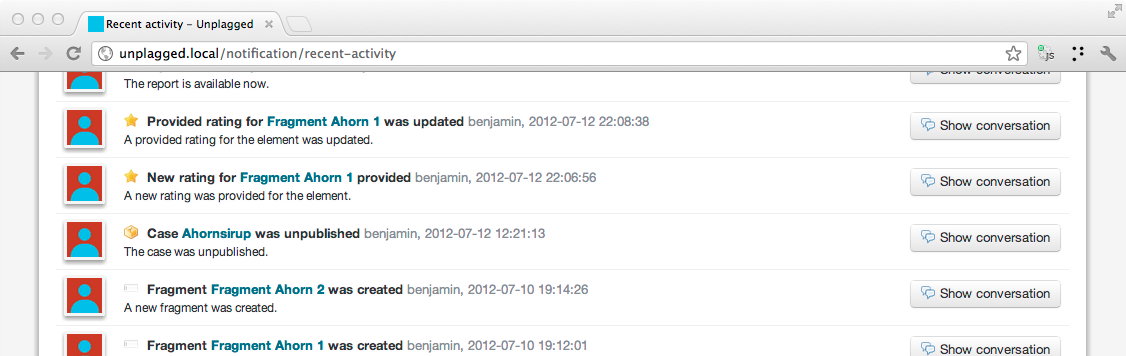
\includegraphics[width=0.97\textwidth]{images/feature-activity-stream.png}
  }
  \caption{Single activity in the activity stream}
  \label{fig:activity-stream-single-activity}
\end{figure}

The following code snippet shows, how to create a new notification when a new automatic plagiarism detection report was created. The static method takes in 3 parameters: a unique name for the notification type, the content object related to the notification and a user object, as the third parameter. A list of all available notification types can either be found in the previousely mentioned actions section or in the scripts/build/initdb.php file, where all notifcation types are being declared.

\begin{lstlisting}[caption=Creating a notification for a created report]
Unplagged_Helper::notify("detection_report_created", $report, $report->getUser());
\end{lstlisting}

Unplagged does have an extensive role and permission management. Therefore the grant on each resource is verified, before it is displayed in the activity stream. Usually the resource related to the notification and the resource the permission check is performed on are the same. Although in some cases, e.g. when rating a fragment, the resource will be the rating itself, but the permission check is done on the fragment. In this case the notify-method is called with a fourth, optional parameter, another resource, in this case the fragment. When the user has access on the fragment, all ratings can be accessed as well, automatically and so are the notifcations.

\subsection{Comments plugin}

Comments are simply a small text related to a specific user and a resource. They can be used to share ideas on a content object collaboratively. The most prominent part at Unplagged, where comments are being used, is the activity stream. A comment can be added by any user having access to the notification. 

\begin{figure}[!h]
  \centering
  \fbox{
    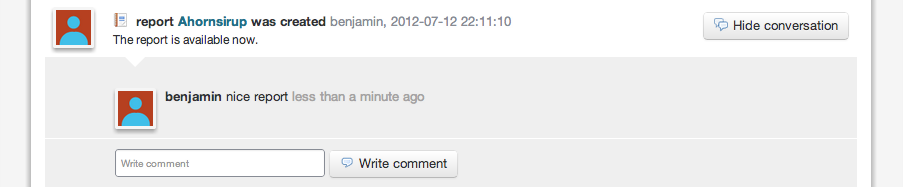
\includegraphics[width=0.97\textwidth]{images/feature-comment.png}
  }
  \caption{Creating a comment on a resource}
  \label{fig:creating-a-comment}
\end{figure}

For providing a better workflow to the user, the comments can be refreshed and added in place. That means, the position where the user scrolled to in the browser does not get affected. The in-place refreshing is realized through AJAX. The comments container is loaded empty and displaying a small loading image only. Not before the user clicks the 'show conversation' button, the comments are being fetched through a post request to the server. Whenever the result is fetched completely, the spinner graphic is hidden and the comments are appended. The parsing of the comments markup is done in Javascript as well. So the server requests are kept small and the server can return JSON only without any HTML.

\begin{lstlisting}[caption=Refreshing the comments of a resource]
	target.show();
      conversation.hide();
      loading.slideDown(800, function() {
        // get the whole conversation
        $.post('/notification/conversation', {
          'source': sourceId
        }, function(data) {
          if(!data.errorcode) {
            conversation.html("");
            $.each(data, function(index, value) {
              conversation.append(renderConversation(value));
            });
            loading.slideUp(800, function() {
              conversation.slideDown(300);
            });
          } else {
            conversation.html('<div class="comment">' + data.message + '</div>');
            loading.slideUp(800, function() {
              conversation.slideDown(300);
            });
          }
        }, "json");
\end{lstlisting}

\begin{lstlisting}[caption=Creating the markup of a single comment]
function renderConversation(data, target) {
    var tpl;
    
    switch(data.type) {
      case 'comment':
        tpl = '<div class="comment">' +
        '<div class="image"><img class="avatar-small" src="' + data.author.avatar + '" /></div>' +
        '<div class="details">' +
        '<div class="title"><b>' + data.author.username + '</b> ' + data.text + 
        ' <span class="date">' + data.created.humanTiming + '</span>' +
        '</div>' +
        '</div>' +
        '</div>';
        break;
    }
    if(!target) {
      return tpl;
    } else {
      target.append(tpl);
    }
  }
\end{lstlisting}

\section{Fragments}

Fragments are the part of the application where found text passages that are plagiairism or potential plagiarism are being documented.

A single fragment contains a candidate and a source document. Each of the two documents is being saved with a starting position (page number / line number combination) and an ending position. These two positions can be used to determine exactly the text being involved in a fragment. To visualize this, the figure \ref{fig:single-fragment}) below shows a sample fragment.

\begin{figure}[!h]
  \centering
  \fbox{
    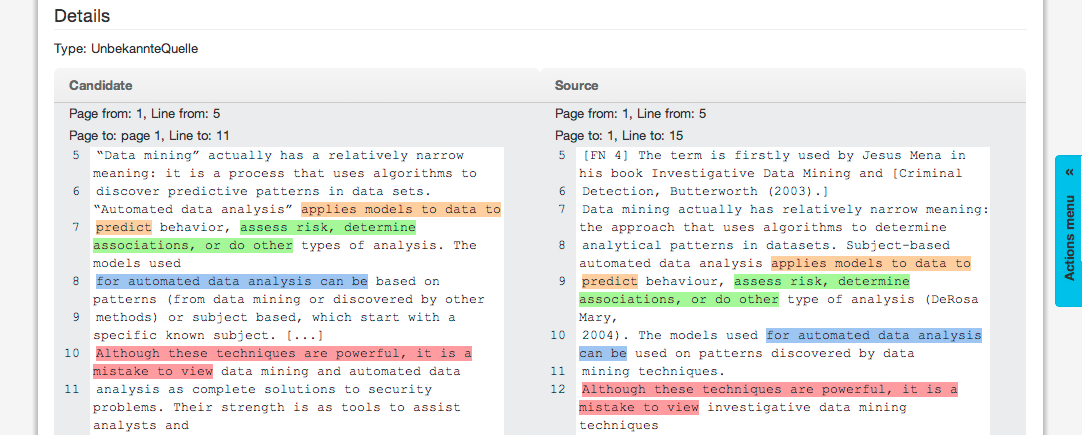
\includegraphics[width=0.97\textwidth]{images/feature-fragment.png}
  }
  \caption{Single fragment with highlighted similarities}
  \label{fig:single-fragment}
\end{figure}

\subsection{Creating a fragment}

Such a fragment can be created in two ways, one for people that like using the mouse and another one that can be used with the keyboard only.

\textbf{The old-fashioned way}

The basic way, which can be accessed through the keyboard only, offers a two-column form to the user where the source and potential plagiarism information can be selected by hand. Once a page or line number is being changed, the text shown below is being updated instantly through AJAX and the similarities are highlighted automatically. Although the big disadvantage of this method is, that the whole page is never displayed and the user actually has to guess where the starting and ending point of the fragment in the text really is. Therefore the values of the line from and line to fields have to be increased or decreased by hand, until they are adjusted properly.

\begin{figure}[!h]
  \centering
  \fbox{
    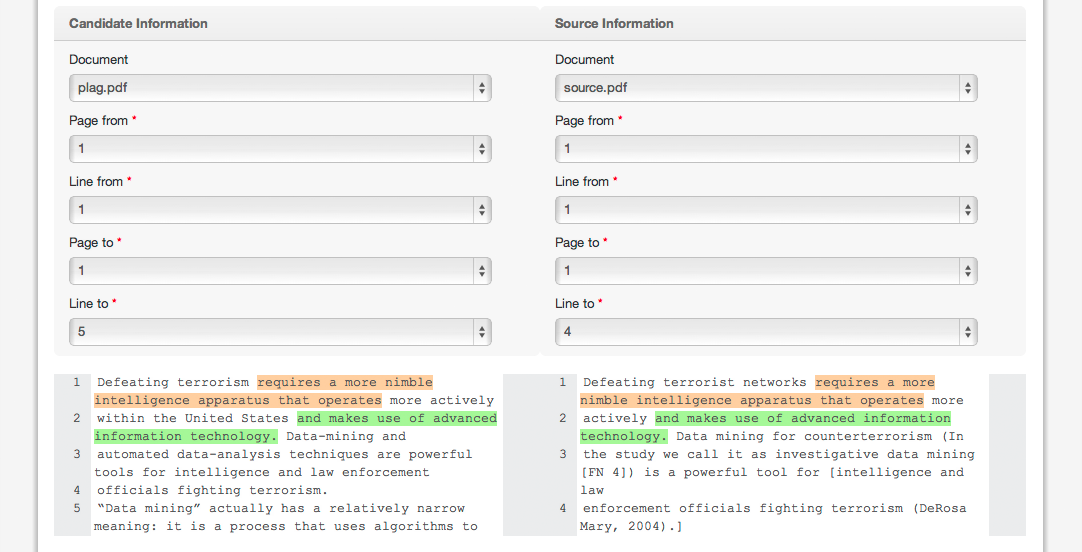
\includegraphics[width=0.97\textwidth]{images/fragment-form.png}
  }
  \caption{Form for creating a fragment by hand}
  \label{fig:fragment-form}
\end{figure}

\textbf{A more comfortable workflow}

Wouldn't it be cool to select text by just marking it with the mouse and having this previousely described form being filled out automatically? We though it would, so we implemented it. 

The user has to go to the document being inspected in the current case, select a page to start with and then hit the button 'Switch to two-column view for fragment creation'. At this point a second document can be selected on the right side and the similarities in both texts are once again being highlighted. (figure \ref{fig:creating-fragment-modern-way-1}) In this two-column view it is also possible to iterate through the pages of the left-side or right-side document to compare page 1 from the left with page 2 from the right and page 1 on the left with page 3 on the right just by one click.

\begin{figure}[!h]
  \centering
  \fbox{
    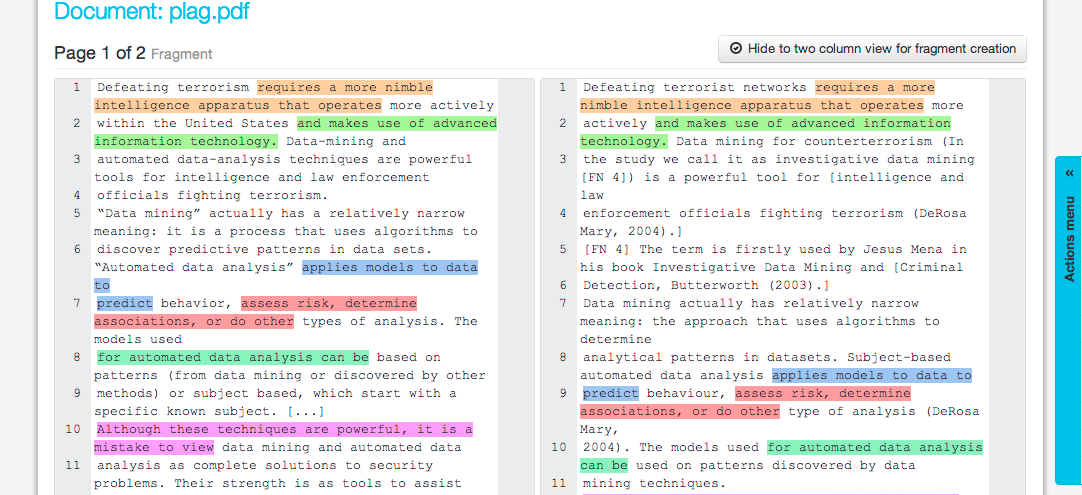
\includegraphics[width=0.97\textwidth]{images/fragment-modern-way-1.png}
  }
  \caption{Creating a fragment the modern way - Step 1}
  \label{fig:creating-fragment-modern-way-1}
\end{figure}

When there are sufficient similarities in an area of the page, a fragment can be created by marking the text, then making a click with the right mouse key to open the context menu and 'set as candidate/source of fragment'. This stores the marked text temporarily until the 'create fragment' button in the context menu is being pressed  (figure \ref{fig:creating-fragment-modern-way-2}). The selection of the 'create fragment' button opens the same form as described in the section before and pre-fills it with the start and end values for page and line for both sides automatically.

This techchnique makes it much easier to create a fragment, since the text can be seen in the context of the whole page, before it is added to the fragment form.

\begin{figure}[!h]
  \centering
  \fbox{
    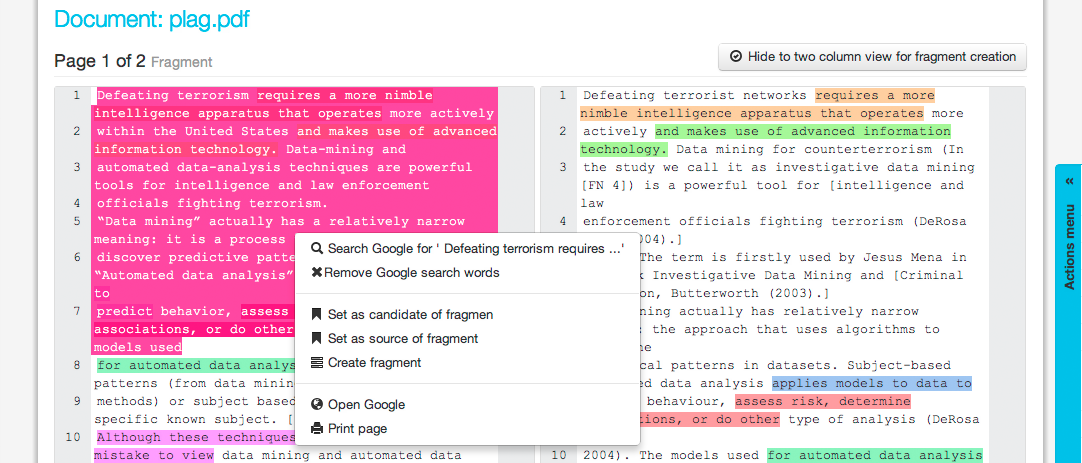
\includegraphics[width=0.97\textwidth]{images/fragment-modern-way-2.png}
  }
  \caption{Creating a fragment the modern way - Step 2}
  \label{fig:creating-fragment-modern-way-2}
\end{figure}

\subsection{Rating a fragment}

A created fragment has to be verified by other collaborators of the case in order to be approved for containing plagiarism. This process is described in the current section.

A rating contains information about the user who made the rating, a flag whether it approves or declines the fragment and an optional property that can contain a description, why the user gave the rating. Each fragment can be approved by a user only once. However the reason and rating type can be changed by the initiator at any time, until the fragment is approved by a certain amount of people. The amount of ratings to lock a fragment and its ratings for further edits is defined in the case administration form. Whenever this amount is reached, the fragment gets locked automatically and can be unlocked by administrators only.

\begin{figure}[!h]
  \centering
  \fbox{
    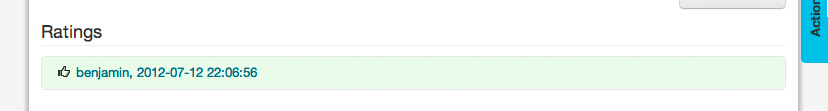
\includegraphics[width=0.97\textwidth]{images/feature-single-rating.png}
  }
  \caption{List of fragment ratings}
  \label{fig:feature-single-rating}
\end{figure}

\section{User avatar}
With the `User avatar' the user gets the possibility to upload a picture to his own profile. Through the function \textit{Profil edititieren}  the user gets to the \textit{Profil editieren} form. 
\pagebreak

\begin{figure}[!h]
  \centering
  \fbox{
    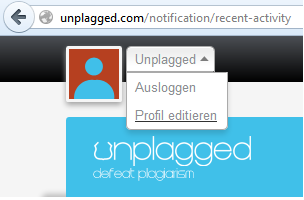
\includegraphics[width=0.97\textwidth]{images/profil_editieren.png}
  }
  \caption{edit profile}
  \label{fig:profil_editieren}
\end{figure}

The uploader in this form allows the user to upload a picture as his avatar.

\pagebreak

\begin{figure}[!h]
  \centering
  \fbox{
    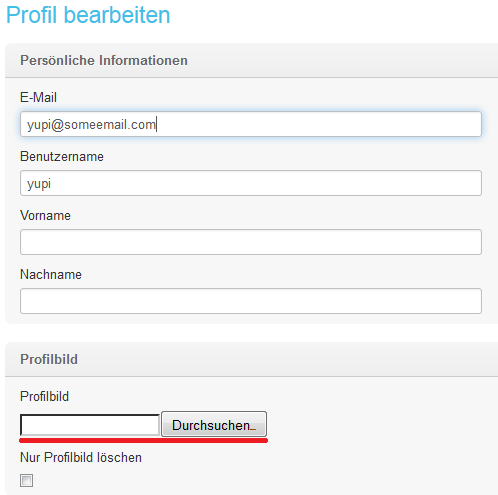
\includegraphics[width=0.97\textwidth]{images/profil_editieren_uploader.png}
  }
  \caption{profile avatar uploader}
  \label{fig:profil_editieren_uploader}
\end{figure}

\pagebreak

After the avatar picture is uploaded the profile picture will be changed.

\begin{figure}[!h]
  \centering
  \fbox{
    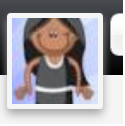
\includegraphics[width=0.97\textwidth]{images/profil_editieren_avatar.png}
  }
  \caption{profile avatar picture}
  \label{fig:profil_editieren_avatar}
\end{figure}


\subsection{Avatar cropping}

While the previous section described how the user avatar can be set, this one explains how the cropping of images that are not in the correct aspect ratio is done. All avatars have to be in a square aspect ratio. However, not all users have the skills to provide an image that meets these requirements. So we decided to crop uploaded images into the appropriate format after they are uploaded.

What we do is taking the shortest of the two rectangle sides and cut a partial from the center of the longer one of the two sides, which has the same length as the shortest side. To make it more visual what that means, figure \ref{fig:cropping-avatar} shows an example. The red area is the part that will be cropped.

\begin{figure}[!h]
  \centering
  \fbox{
    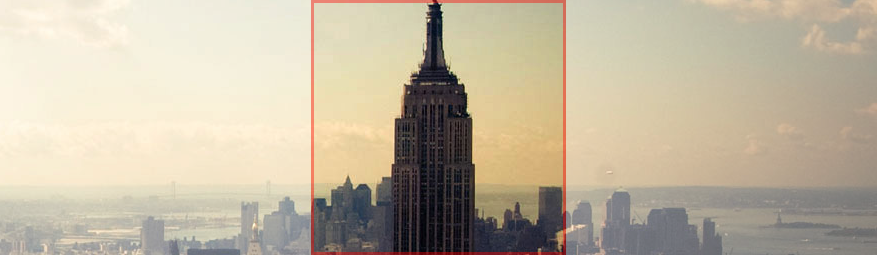
\includegraphics[width=0.97\textwidth]{images/cropped-avatar.png}
  }
  \caption{Cropping avatar}
  \label{fig:cropping-avatar}
\end{figure}

The cropped image then is scaled to the needed width and height, currently 50 x 50 pixels. The algorithm for cropping that has been developed, is shown in the following code snippet.

\begin{lstlisting}[caption=Cropping an image to a square aspect ratio]
public function crop($thumbWidth, $thumbHeight){
    //getting the image dimensions
    list($width, $height) = getimagesize($this->file->getFullPath());
    
    //saving the image into memory (for manipulation with GD Library)
    $myImage = imagecreatefromjpeg($this->file->getFullPath());

    // setting the crop size
    if($width < $height) {
      $twidth = $width;
      $theight = $width;
      $x = 0;
      $y = $height / 2. - $width / 2.;
    } else {
      $twidth = $height;
      $theight = $height;
      $x = $width / 2. - $height / 2.;
      $y = 0;
    }

    // creating the thumbnail
    $thumb = imagecreatetruecolor($thumbWidth, $thumbHeight);
    imagecopyresampled($thumb, $myImage, 0, 0, $x, $y, $thumbWidth, $thumbHeight, $twidth, $theight);

    imagejpeg($thumb, $this->file->getFullPath());

    imagedestroy($thumb);
    imagedestroy($myImage);

    return $this->file;
  }
\end{lstlisting}


\section{Automatic Plagiarism Detection Webservices}

Unplagged itself is a workbench, where the plagiairism detection is done by hand. Although it provides useful automatic tools that help the user to make the process of plagiairism detection easier. One of these tools are external webservices that check a specific text for plagiairism and try to find sources which can be used for further inspections.

We were talking to 3 companies offering such a webservice: Docoloc, PlagScan and PlagAware. As a proof of concept the PlagAware webservice has been implemented and added to our application, it will be described in the following section.

\subsection{PlagAware}

PlagAware, a website for automatic plagairism detection is a commercial website which costs money depending on the amount of text to analyze. It figures out possible sources of the text handed in on their website and creates a PDF report with a list of all the found sources (figure \ref{fig:plagaware-result}).

\begin{figure}[!h]
  \centering
  \fbox{
    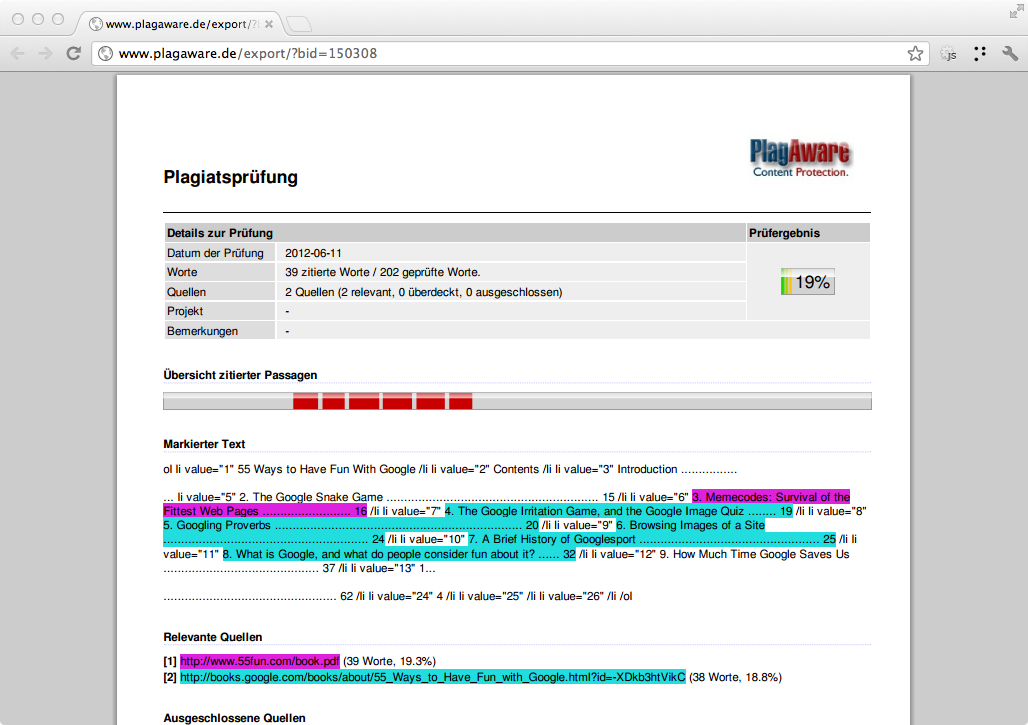
\includegraphics[width=0.97\textwidth]{images/feature-plagaware-result.png}
  }
  \caption{PlagAware result document}
  \label{fig:plagaware-result}
\end{figure}

The website also offers a webservice which takes text as input and notifies the user when the analyzing is finished. Although it does not provide any information about the sources through the webservice response call, there is only a status code and the percentage of plagairism responded. Whenever the response was sent, the user has to go to the PlagAware website and check out the detailed results there.

Since the PlagAware webservice is a simple HTTP-Webservice, the connection is done through an HTTP request with curl.
\begin{lstlisting}[caption=Sending a request through curl to the PlagAware webservice]
public function detect(Application_Model_Document_Page_DetectionReport &$report){
    $url = "http://www.plagaware.de/service/submittext";
    $fields = array(
      'UserCode'=>urlencode($this->paUserCode),
      'ResultUrl'=>urlencode($this->paResultUrl . $report->getId()),
      'TestText'=>urlencode($report->getPage()->getContent()),
      'DryRun'=>urlencode($this->paDryRun)
    );

    // url-ify the data for the POST
    $fields_string = "";
    foreach($fields as $key=>$value){
      $fields_string .= $key . '=' . $value . '&';
    }
    rtrim($fields_string, '&');

    $ch = curl_init();
    curl_setopt($ch, CURLOPT_URL, $url);
    curl_setopt($ch, CURLOPT_RETURNTRANSFER, 1);
    curl_setopt($ch, CURLOPT_CONNECTTIMEOUT, 10);
    curl_setopt($ch, CURLOPT_POST, count($fields));
    curl_setopt($ch, CURLOPT_POSTFIELDS, $fields_string);

    $output = curl_exec($ch);
    $info = curl_getinfo($ch);
    curl_close($ch);
}
\end{lstlisting}

The response is sent through a GET-Request to a pre-defined request URL, in our case '/document/response-plagiarism/report/<report-id>'. The call of this action stores the result in our database and creates a notifcation for the user, indicating that a new report is available.

\section{Permission and role management}

Unplagged does offer an extensive permission and role management, which controls access to pages and entities within the system. It contains two important parts: roles and permissions. A permission is a actually a single right on a resource within the portal and roles are collections of permissions.

\subsection{Roles}

Roles are being used for assigning pre-defined sets of permissions to a single user in different situations. There exist 4 different types of roles, with different characteristics:

\begin{itemize}
\item    	Global roles
\item   	User roles  
\item    	Case default roles
\item   	Case roles
\end{itemize}

Besides the different role types, there exists a concept of role inheritance in our system. One role can inherit from another one, in this case, a user does have the joined rights of the main role and the inherited role as well. 

\textbf{Global roles}

To make this more visual, let's start with the global roles. Global roles include default roles for guests, registered users and admins. A non-registered user does have the guest role by default, a registered user the user role. Since administrative users need some more privilleges, they need the admin role as well. Since the admin role is an inheritable role, it extends the user role and user get's all the rights which are either in the user role or in the admin role.

\textbf{User roles}

When a user registeres on the plattform, a copy of the global user role is created and assigned to the user as it's default role. This role can be modified for each user without influencing other users, so one user can have completely different rights than another one.

\textbf{Case default roles}

All the permissions defined in the roles described above are related to all cases the user is taking part in. Although often it is necessary to add different rights to a user in different cases. For example in one case a user can access all documents, in another one the user can access the files area only. For this case two case default roles are provided: an admin role and a collaborator role, they can be seen as a global role on the case level, used as templates for all cases. 

\textbf{Case roles}

When a new case is created, the same process as described for the user roles takes part, a copy of the case default roles is created, they can be assigned to any collaborator of the case (figure \ref{fig:collaborators-form}). A case role can be added to a user by accessing the Case > Edit form in the 'case collaborators' section. An autocompletion field let's the user search for collaborators by username and then through a dropdown, the role can be selected, as shown in figure \ref{fig:collaborators-form}.

\begin{figure}[!h]
  \centering
  \fbox{
    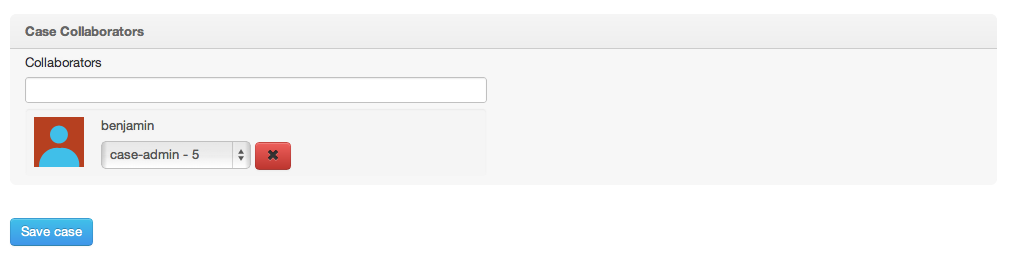
\includegraphics[width=0.97\textwidth]{images/collaborators-form.png}
  }
  \caption{Roles overview}
  \label{fig:collaborators-form}
\end{figure}

All the different roles used in Unplagged can be managed in the Administration > Roles area (figure \ref{fig:roles-list} and figure \ref{fig:roles-form}).

\begin{figure}[!h]
  \centering
  \fbox{
    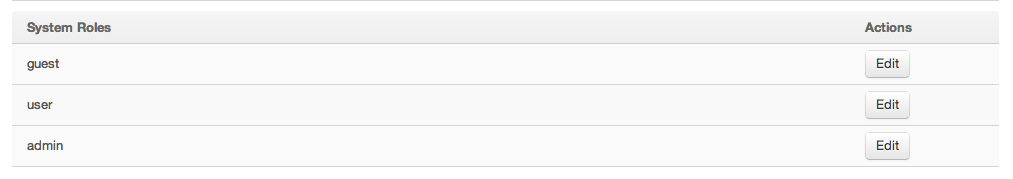
\includegraphics[width=0.97\textwidth]{images/roles-list.png}
  }
  \caption{Roles overview}
  \label{fig:roles-list}
\end{figure}

\begin{figure}[!h]
  \centering
  \fbox{
    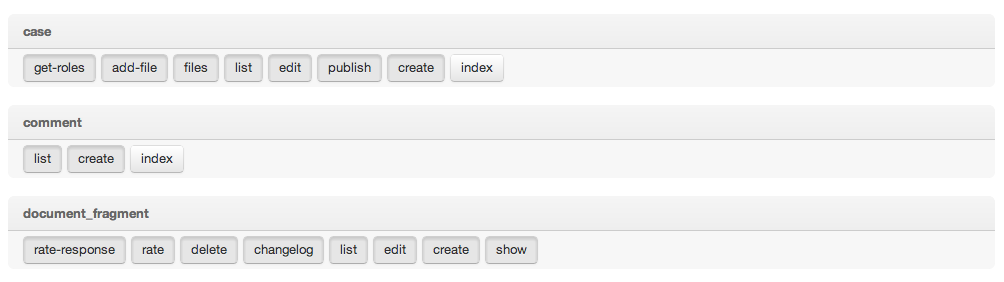
\includegraphics[width=0.97\textwidth]{images/roles-form.png}
  }
  \caption{Role form}
  \label{fig:roles-form}
\end{figure}

\subsection{Permission types}

There exist two permission types which are extending from an abstract permission model – page permissions and model permissions. How they differ from each other will be described further on. Usually a permission is related to a specific object, but we also do have global permissions, which define access to all entities of a kind. 

A single permission basically contains four properties:

\begin{itemize}
\item      type – what model / page type is protected (e.g. document, file, case) 
\item      action – what action of the type (e.g. read, list, create)
\item      base – which entity is protected (e.g. a real entity id or a * for global rights)
\item      permission type – page permission or model permission
\end{itemize}

When a user does not have access to a page resource or a model resource, one is redirected to the previously accessed page automatically.

\textbf{Model permissions}

The ModelPermission entity manages access to single objects within the system, this includes for example cases, files, documents, fragments and comments. Each of them currently has a fixed set of permission actions, based on the CRUD design pattern – create, read, update, delete and a fifth one called authorize. The authorize permission allows a user to control the permissions on a specific entity.

If the user does have the authorize permission on an entity, the form to edit them, can accessed through the actions menu in the list view of the object, as shown in figure \ref{fig:add-model-permission}. 

\begin{figure}[!h]
  \centering
  \fbox{
    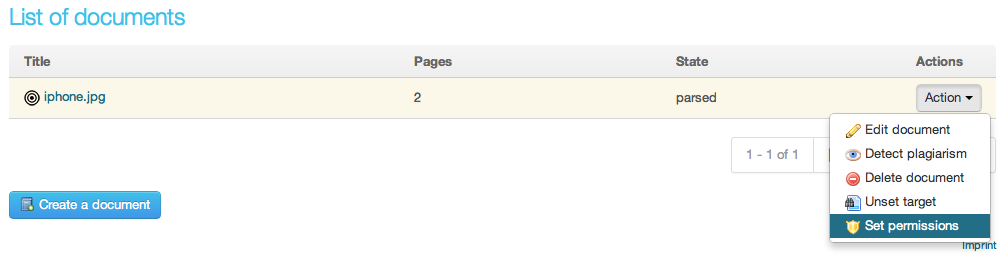
\includegraphics[width=0.97\textwidth]{images/add-model-permission.png}
  }
  \caption{Access form for editing model permissions}
  \label{fig:add-model-permission}
\end{figure}

The form provided to set the permissions offers an autocompletion textfield at the top, where usernames can be searched and afterwards the permissions can be defined by enabling or disabling the buttons below the username (figure \ref{fig:set-model-permissions}).

\begin{figure}[!h]
  \centering
  \fbox{
    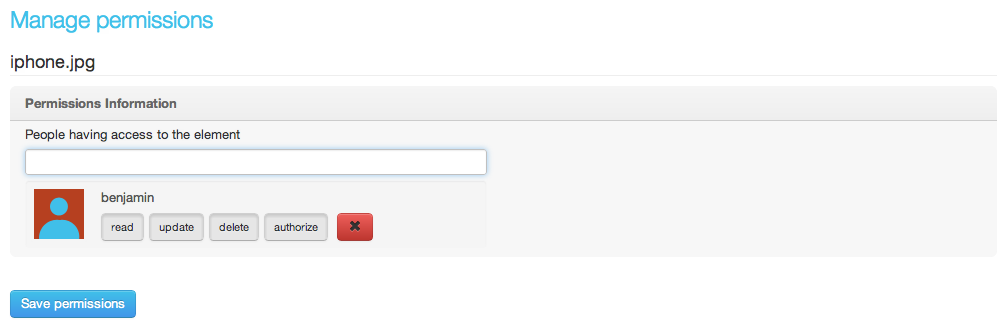
\includegraphics[width=0.97\textwidth]{images/set-model-permissions.png}
  }
  \caption{Set permissions on an entity}
  \label{fig:set-model-permissions}
\end{figure}

The permission check on models does have to be done by hand in any controller action, where needed. A simple selection of the required permission and then a call of the hasPermission-method on the user role is sufficient. The following example checks the users read permission on a specific document:

\begin{lstlisting}[caption=Checking the user permission on an entity]
$permission = $this->_em->getRepository('Application_Model_ModelPermission')->findOneBy(array('type'=>'document', 'action'=>'read', 'base'=>$document));
if(Zend_Registry::getInstance()->user->getRole()->hasPermission($permission)){
	// user has access
}
\end{lstlisting}

\textbf{Page permissions}

The second type of permissions are the page permissions. They control access to controller and action methods. This means, they define whether a user can for example access the page /document/list or not. The available permissions are being generated on each deployment of the site automatically. So when a new action in a controller is created, it will be available as a new permission after the next deployment.


\section{Barcode}
The barcode is a visual representation of the amount of plagairism in each page of the target document. In our application it is used in two representations, which use the same data source but have another visual layout and details shown within.

The barcode has 4 different colors, which represent another amount of plagairism within the page:

\begin{itemize}
\item      light blue: the page is disabled for the barcode
\item      white: page not available or no plagiarism
\item      black: more than 0 percent plagiarized
\item      dark red: more than percent plagairized
\item      light red: more than percent plagairized
\end{itemize}

\textbf{Representation with labels on the home page}

The first representation can be found at the home page, here are the barcodes of all published cases being displayed. The barcode is being displayed with page numbers below and the width is dynamic, so the barcode increases when the page gets wider and the barcode gets smaller, when the page width decreases. 

\begin{figure}[!h]
  \centering
  \fbox{
    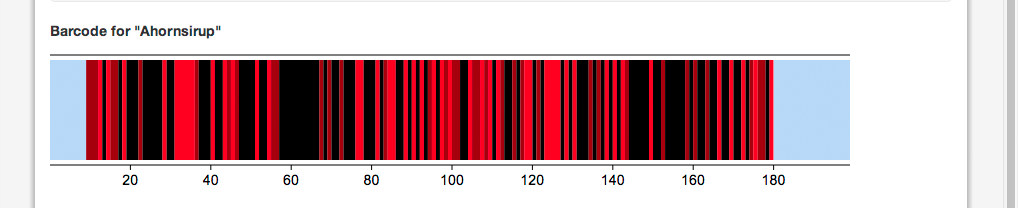
\includegraphics[width=0.97\textwidth]{images/feature-barcode-website.png}
  }
  \caption{Barcode on home page}
  \label{fig:feature-barcode-website}
\end{figure}

Since this mechanism is very dynamic, an algorithm needed to be developed to calculate the x axis values taking into consideration the page width and the number of pages in the document being visualized. It assumes that a label needs at least 45px of width and the whole barcode has to look well to a width of 500px.

So what we do is, we start with a setpsize of 10 for the page numbers: 10 20 30 40 50, now we check if the amount of pages can be displayed with such a fine scale to stay in the 500px range. For example a page count of 200 leeds to 20 values on the x axis and if we assume 45px are necessary to display a value on the axis properly, we would need 900px of width, but we have only 500px available. Otherwise we would have crossovers when we get below 900px. So the stepsize is increased by 10, until we stay in the 500px maximum width. As it turns out, a step size of 20 pages is sufficent to get a width of 450px in the end. The code for this calculation is being shown below.

\begin{lstlisting}[caption=Generating the barcode x axis]
private function generateAxis() {
        $labelStepsize = 10;

        while (true) {
            $count = sizeof($this->pages);
            $labelCount = floor($count / $labelStepsize);

            // we assume a label needs 45px and 500px is the width that needs to be displayable without crossovers
            if (45 * $labelCount > 500) {
                $labelStepsize += 10;
                continue;
            }
            break;
        }

        $label = $labelStepsize;
        $x = 0;
        while ($x < ($this->width - ($this->initWidth * $labelStepsize))) {
            $x += ($this->initWidth * $labelStepsize);
            $this->result .= '<text x="' . $x . $this->widthUnit . '" y="' . $this->y . '" font-family="Arial" font-size="14" text-anchor="middle">' . $label . '</text>';
            $this->result .= '<line x1="' . $x . $this->widthUnit . '" y1="' . ($this->y - 20) . '" x2="' . $x . $this->widthUnit . '" y2="' . ($this->y - 15) . '" stroke-width="1" stroke="#000000"></line>';

            $label += $labelStepsize;
        }
    }
\end{lstlisting}

\textbf{Representation without labels in the report}

The second area where barcodes are used, are the final reports. They will be explained in the next section. The space available in the PDF is much less than on the website and the library we are using for generating the PDF report does not support text in scable vectors graphics, so we decided to display the barcodes without labels for now. However the data visualized is exactly the same.

\pagebreak

\section{Report}

The report is needed to collect and document all the found plagiarized fragments of the reviewed document. It will be used as an evidence to proof (major) plagiarism.
The report documents all founded plagiarized parts including the corresponding sources.

The report has also a barcode on the first page to give the reader a quick visuell overview to the plagiarism level of the reviewed document.

Below you can read about the generation of a report, a short description of the development and the outlook of an example of a report.

\subsection{Generating of a report}

To generate a report it is neccessary that there exist approved fragments for this case. Without approved fragments in a case it is not possible to generate a report for this case. 
This is made to have only approved fragments listed in the report. This makes sure that only real plagiarized textparts are listed in the report.

To generate a report the user needs to choose the tab \textit{Berichte} and than click at the button \textit{Bericht erstellen}. After the user clicked at the  button \textit{Bericht erstellen} it has the possibility to fill up the report form to give the title of the report and to give some evaluations about the reviewed document.

\begin{figure}[!h]
  \centering
  \fbox{
    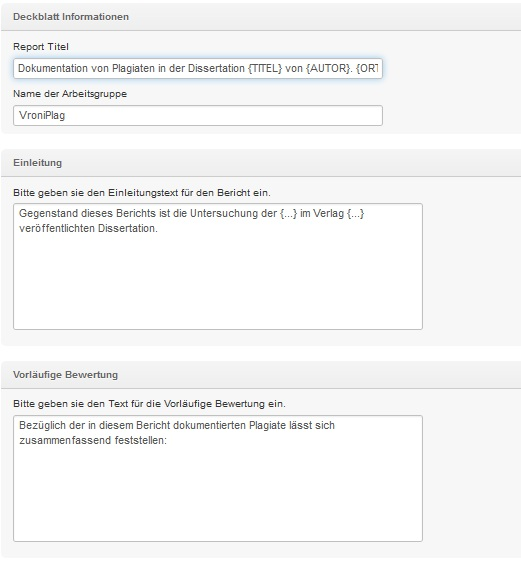
\includegraphics[width=0.97\textwidth]{images/report_form.jpg}
  }
  \caption{report form}
  \label{fig:report_form}
\end{figure}

\pagebreak

After the user saved the entries of the form the report will be generated and will be listed.

\begin{figure}[!h]
  \centering
  \fbox{
    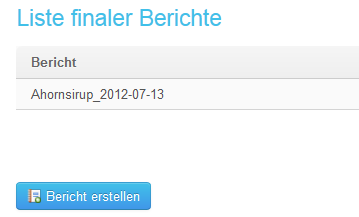
\includegraphics[width=0.97\textwidth]{images/report_list.png}
  }
  \caption{example of a listed report}
  \label{fig:report_list}
\end{figure}

\subsection{The developing of the report function}

Before the start of the actual development of the report function, it was necessary to first make researches about pdf generation frameworks. After some researches and hints from unplagged group members the decision felt to \textit{dompdf}. 

\subsubsection{Dompdf}

\textit{Dompdf} is an easy to use framework which gives users the posibility to generate pfd files dynamically. After the familiarisation phase it was not difficult to use this framework to generate the first report in pdf form. \textit{Dompdf} had problems with pagebreaks. Reasons were for example that it could not handle it if the content between two \textit{div tags} or a \textit{table cell} was longer than one page.
But there was another big disadvantage of \textit{dompdf}, it was not possible to represent the fragments in column form. It was only possible to show the fragments on the generated report among one another. This was a known problem of \textit{dompdf}.

After a lot of tryings to code workarounds and make researches in forum, it was obvious that there was no way to make the column representing that we needed for the fragments view, that will be shown in the report, with the \textit{dompdf} framework. At the end it was necessary to make that not easy decision to pass on \textit{dompdf} and to find a framework that suits our needs better.
So another research round was necessary. This time we knew better what we were searching for. First of all a framework which can handle column representation.

Because of this and some other reasons the report generating framework \textit{html2pdf} is used.

\subsubsection{Html2pdf}

\textit{Html2pdf} is the choosed framework for the report generation. The big advantage of \textit{html2pdf} was that it gives the possibility to show the fragments in column form. Another big advantage is that with \textit{html2pdf} it is possible to add svg code to the html content and therefor include it to the generated pdf file. The svg possibility was necessary to add the barcode in the report which was generated as svg.

For the barcode generation of the report the following code is used.

\begin{lstlisting}[caption=Generating the barcode for the report]
  private function getBarCode($case) {
        $str_svg = $case->getBarcode(80, 150, 100, false, '%')->render();
        $str_svg = str_replace('svg', 'draw', $str_svg);
        $str_svg = str_replace('width=', 'w=', $str_svg);
        $str_svg = str_replace('height=', 'h=', $str_svg);

        return "<h2>Barcode</h2>" . $str_svg;
    }
\end{lstlisting}

The pagenumbers are written in the footer. The pagenumbers are generated with the following code.

\begin{lstlisting}[caption=Generating the pagenumbers]
    private function getFooter($pagenumber) {
        return "<page_footer>" . $pagenumber . "/%pagenumber%</page_footer> ";
    }
\end{lstlisting}

The use of \textit{html2pdf} class is shown below.

\begin{lstlisting}[caption=Use of the class html2pdf]
        $html2pdf = new HTML2PDF('P', 'A4', 'en');
        $html2pdf->WriteHTML($content);
\end{lstlisting}

The following code is a workaround. This workaround is necessary because \textit{html2pdf} has pagebreak problems. This problem was also found in \textit{dompdf}. This problem was not so easy to solve than thought at the beginning. The problem here is that  \textit{html2pdf} needs always proper and valid html content. From this content the pdf file will be generated. Valid html content means also that all html tags need to be closed. 

For the coloured simtext passages span tags are used. This span tags contains the plagiarized text. If the content of the span tags are seperated in two or more pages than the span tag can not be closed within one page. This means for \textit{html2pdf} it is not valid html anymore and \textit{html2pdf} refuses to generate the pdf file.

The workaround limits the words which will be written in one page of 400 words, if there is a span tag which is not closed it will be closed then.

\begin{lstlisting}[caption=Workaround for the \textit{html2pdf} pagebreak problem]
   /**
     * Removes the multiple blank spaces from the given parameter.
     */
    private function remove_spaces($text) {
        while (true) {
            $replaced = str_replace('  ', ' ', $text);
            if ($replaced != $text) {
                $text = $replaced;
            } else {
                break;
            }
        }
        return $text;
    }

 /**
     * Cuts the given text into an array, which each element contains
     * $nbWordsProPage words.
     */
    private function cut_text_into_pages($text) {
        $text = $this->remove_spaces($text);
        $exploded = array_slice(explode(' ', $text), 0);
        $nbWordsProPage = 400;
        $nbPage = 0;
        $pages = array();
        $rest = "";
        $nbRest = 0;

        for ($i = 0; $i < sizeof($exploded); $i+=$nbWordsProPage) {
            $page = $rest . implode(' ', array_slice($exploded, $i, $nbWordsProPage - $nbRest));
            $result = $this->check($page);
            $rest = $result["toRetrieve"] . " ";
            $nbRest = str_word_count($rest);
            $pages[$nbPage++] = $result["s"];
        }

        return $pages;
    }

    private function result($length, $s) {
        $array = array();
        $array["toRetrieve"] = substr($s, $length, strlen($s) - $length);
        $array["s"] = substr($s, 0, $length);
        $array["original"] = $s;
        return $array;
    }

    private function check($s) {
        $nbST = substr_count($s, ST);
        $nbBT = substr_count($s, GT);
        if ($nbST == $nbBT) {
            $nbSpanOpen = substr_count($s, SPAN_OPEN);
            $nbSpanClose = substr_count($s, SPAN_CLOSE);
            if ($nbSpanOpen == $nbSpanClose) {
                return $this->result(strlen($s), $s);
            } else {
                // 'halli hallo <span>'
                return $this->result(strrpos($s, SPAN_OPEN), $s);
            }
        } else {
            // one tag is not closed
            //'halli hallofff <span></span'
            //'halli hallofff <span'
            $nbSpanOpen = substr_count($s, SPAN_OPEN);
            $nbSpanClose = substr_count($s, SPAN_CLOSE);

            return $this->result(strrpos($s, SPAN_OPEN), $s);
        }
    }
\end{lstlisting}

\subsection{Outlook of a report}

The report has besides his first page, three further parts. The defaulttext with the evaluationtext, the list of approved fragments and the references to the according sources.

\begin{figure}[!h]
  \centering
  \fbox{
    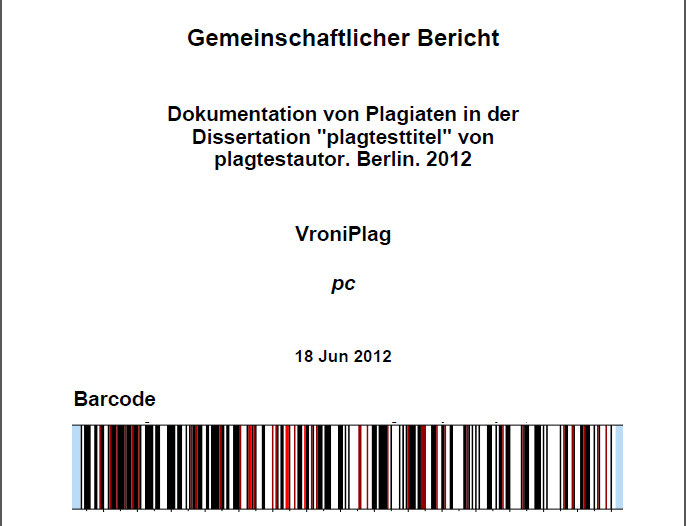
\includegraphics[width=0.97\textwidth]{images/report_deckblatt.png}
  }
  \caption{example of a first page of a report}
  \label{fig:report_deckblatt}
\end{figure}

\pagebreak

The defaulttext also can contain evaluationtext, this is individual text which was given from the person who generated the report, through the report form.
\pagebreak

Below there is an example of the defaulttext.

\begin{figure}[!h]
  \centering
  \fbox{
    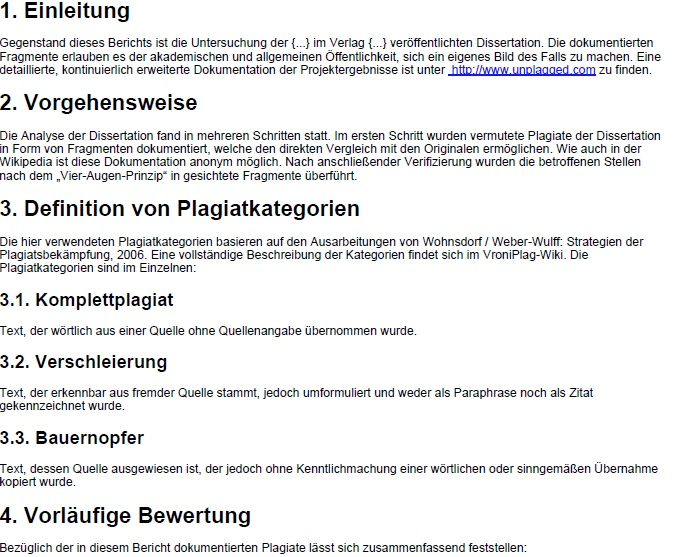
\includegraphics[width=0.97\textwidth]{images/report_default_evaluation_text.jpg}
  }
  \caption{report defaulttext}
  \label{fig:report_default_evaluation_tex}
\end{figure}
\pagebreak

After the evaluation text the list of approved fragments will be shown.

\begin{figure}[!h]
  \centering
  \fbox{
    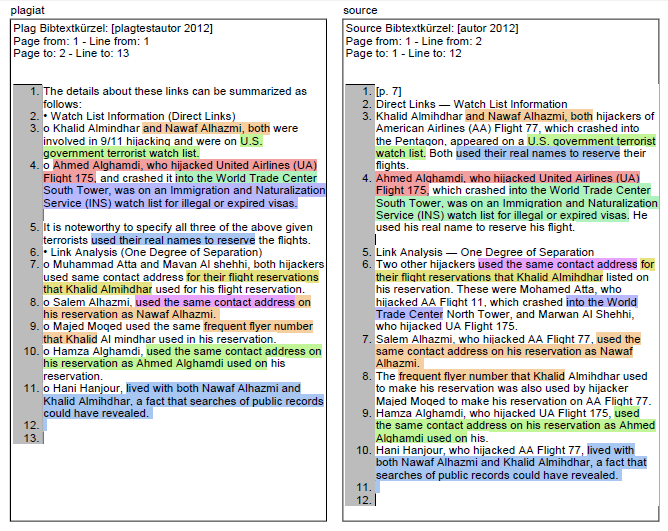
\includegraphics[width=0.97\textwidth]{images/report_fragment.png}
  }
  \caption{example of a listed approved fragment}
  \label{fig:report_fragment}
\end{figure}

\pagebreak
At the end all the references to the found sources are mentioned.

\begin{figure}[!h]
  \centering
  \fbox{
    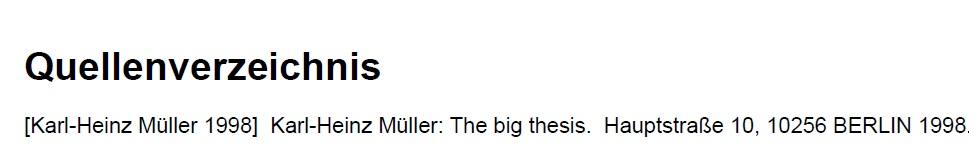
\includegraphics[width=0.97\textwidth]{images/report_according_sources.jpg}
  }
  \caption{example of a listed source}
  \label{fig:report_according_sources}
\end{figure}

\pagebreak

\section{Simtext}
Simtext is a common name about a tool which helps to check for text similarity between two inputs. This tool uses complex algorithm to compare the inputs. The result of the comparison is an output which should contain similar text passages between the two inputs and the positions of the text passages on the documents. 

There are many softwares for text similarity tester, but at the beginning of the development for simtext in our workbench, we used the software SIM of Dick Grune. This software is free and the result after the comparison process is reliable. We integrated this software to Unplagged but there were some disadvantages about this software. Then we saw that the Vroniplag community had developed a simtext tool, which was also based on SIM, but cleverly modified in Javascript. This version was quite simplified and optimized for web browser. We would like to adapt this Javascript version in our workbench as well, but unfortunately it was not that easy to integrate it. The reason was that some of its functions were not suitable in our environment at all. Therefore we decided to modify this Javascript version in PHP. 

Here are some descriptions about the development and improvement of simtext tool for our workbench.

\subsection{SIM in C - Original version}
The program was developed by Dick Grune. It was written in C and runnable in other languages like Java, Pascal… and had a quite complicated structure. 

''The general outline of the similarity checker is as follows:


\begin{enumerate}
\item the files are read in (pass 1)
\item a forward-reference table is prepared
\item the set of interesting runs is determined
\item the line numbers of the runs are determined (pass 2)
\item the contents of the runs are printed in order (pass 3)''
\end{enumerate}
%\footnote{ftp://ftp.cs.vu.nl/pub/dick/similarity_tester/TechnReport - Date: 24.07.2012}

The result of the comparison process was a plain text file which showed the similar text passages and the positions, where the plagiarized text was similar with the source text.

We integrated this software into our workbench, but because it was not specifically developed for web, there were some disadvantages of this software. They are:

\begin{itemize}
\item it was complicated to run the program  - It had to be compiled through the C command 
\item input/output were plain text files
\item there was no color for marking the similar text passages
\item only similar text passages were shown, not the whole documents
\item the result was simple and monotone and not impressive
\item In order to compare HTML texts or other file types, it  was maybe needed to parse the inputs in plain text files. After comparing, the result as plain text file should be parsed again in HTML so that it can be performed in the browser. Therefore the comparison process was complicated and the speed could be decreased if there were a lot of documents.
\end{itemize}

\begin{figure}[!h]
  \centering
  \fbox{
    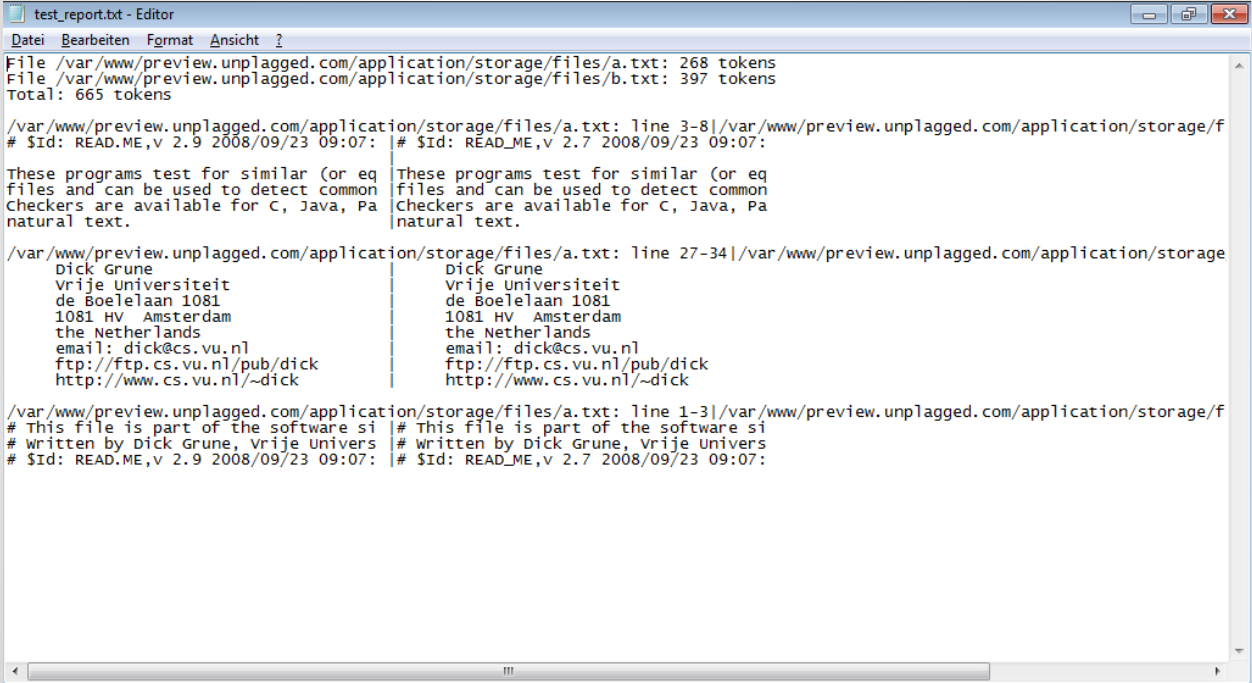
\includegraphics[width=0.97\textwidth]{images/SIM_Dick_Grune.png}
  }
  \caption{Simtext in C}
  \label{fig:Sim_in_C}
\end{figure}

\subsection{Vroniplag’s Javascript version}
We found out that Vroniplag also had its own text comparison tool, which was written in JavaScript. According to the author, this web-based version was also based on the original version of Dick Grune. % \footnote{http\://de.vroniplag.wikia.com/wiki/Benutzer\:Marcusb/Farbige\_Fragmente - Date\: 24.07.2012}

The Javascript version could compare two fragments, finds out the similar text passages and marks them with different colors. A text passage is defined by default as a phrase which is more than 4 tokens (words) long.

We thought this version was more flexible. Besides the text comparison function, it was also possible to mark the similar text passages with different colors. This could help the user get a better overview about the result. Because it was written in Javascript, it could also read the HTML texts and compare them directly without the parsing process as in the SIM version above. In addition, there was a button which could be switched on/off to show/hide the colors.

But when we tried to adapt this version to our workbench, there were some difficulties that we thought the adaptation was too complicated. The difficulties were:
\begin{itemize}
\item Because Vroniplag is a Wiki-Community, so the version was written and adjusted to this Wiki’s environment. That means, the author has customized the version so that it fit to the Wiki page’s attributes. There were a lot of the author’s improvements and changes of relative functions only for the purpose that it could work in Wiki. Therefore it was not easy to adapt the version again in our workbench, because we did not have the suitable conditions as by Wiki
\item If the user does not have/want Javascript turned-on on the browser, it would be difficult to see the colored result of the text comparison tool
\item We wanted to make our own thing
\end{itemize}

\begin{figure}[!h]
  \centering
  \fbox{
    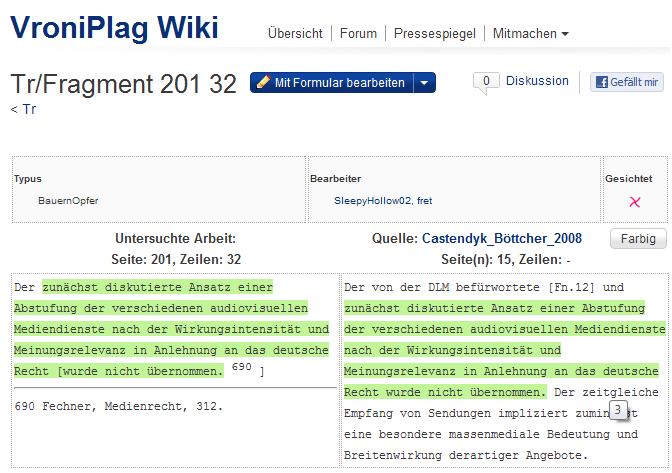
\includegraphics[width=0.97\textwidth]{images/vroni_farbfrag.png}
  }
  \caption{Vroniplag Colored Fragments}
  \label{fig:Vroniplag_Colored_Fragments}
\end{figure}

\subsection{Unplagged’s PHP version}
After considering advantages and disadvantages of the two versions, we decided to modify the Javascript version in PHP language. Because of the disadvantage of the Wiki’s environment, we took only the main part of the Javascript version - the text compare function - and tried to modify it to our workbench.

\subsubsection{Text comparison function}

We tried to figure out how the text comparison function works. First we just ''translated'' every code line from Javascript into PHP. It was not difficult to rewrite the code, but it took much time and effort to find and fix the errors. We had to debug most of  the code lines. In some cases we found out that it did not work because some issues seem to be the same thing in both languages, but actually if they were written in PHP, they had a different meaning than if they were written in Javascript.

For example we had to check, if a key named \textit{match\_tag} existed in a hash table named \textit{match\_table}. If yes, the value for this key will be added. In the JavaScript version, they used \textit{if (match\_tag in match\_table)}, where it did not matter if \textit{match\_tag} was a key or a value. In PHP version, the equivalent function \textit{if(in\_array(\$match\_tag, \$match\_table))}, was used. We thought it would be the same thing like in Javascript, but the result we received was always an empty array. After several times debugging we realized that it was about an associative array in PHP and this function searched only for the value. We had to check for the key and \textit{if(array\_key\_exists(\$match\_tag, \$match\_table))} had worked finally.

Another example for the diversity of the same issues in different languages was the different meaning of NULL. In Javascript NULL means an object with no initial value, in PHP it means 0, empty or false (3). So there were some places in the code declared with NULL, it should be changed to -1 in PHP (we chose -1, just a different value, sothat it would not return to an empty object, which we did not have in the code) in order to receive the expected result. 
\footnote{http://php.net/manual/en/types.comparisons.php}

After fixing all the errors, we got a nice text comparison function in PHP. The final result is an array of token lists in the form:

\begin{lstlisting}
array{doc_1, start_token_1, doc_2, start_token_2, length} 
\end{lstlisting}

where doc\_X are indices into the documents array, and start\_token\_X are indices into the respective token list of the documents, length is the default length of a phrase. 
\footnote{http://de.vroniplag.wikia.com/wiki/MediaWiki:Fragcolors/code.js}

For example we had two dummy inputs

\begin{figure}[!h]
  \centering
  \fbox{
    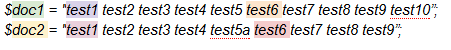
\includegraphics[width=0.97\textwidth]{images/sim_ex_1.png}
  }
  \caption{simtext result}
  \label{fig:simtext _result}
\end{figure}

Here was the matches

\begin{figure}[!h]
  \centering
  \fbox{
    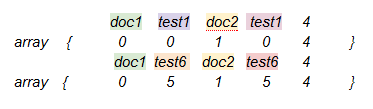
\includegraphics[width=0.97\textwidth]{images/sim_ex_2.png}
  }
  \caption{simtext result}
  \label{fig:simtext_result}
\end{figure}
The result was presented on browser

\begin{figure}[!h]
  \centering
  \fbox{
    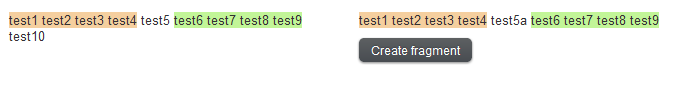
\includegraphics[width=0.97\textwidth]{images/sim_result.png}
  }
  \caption{simtext result}
  \label{fig:report_deckblatt}
\end{figure}

\subsubsection{Disadvantages of the text comparison function}

The first disadvantage of the text comparison function was maybe the restriction of the length of a phrase. By default a phrase was a list of tokens which was more than 4 tokens. That means it could be difficult to find out plagiarized positions if their length was less than 4 tokens. 

Another disadvantage was that the strict comparison algorithm could compare only continual phrases. That means if at some positions there was a tiny change such as a break line or a comma, the algorithm could miss them.

\begin{figure}[!h]
  \centering
  \fbox{
    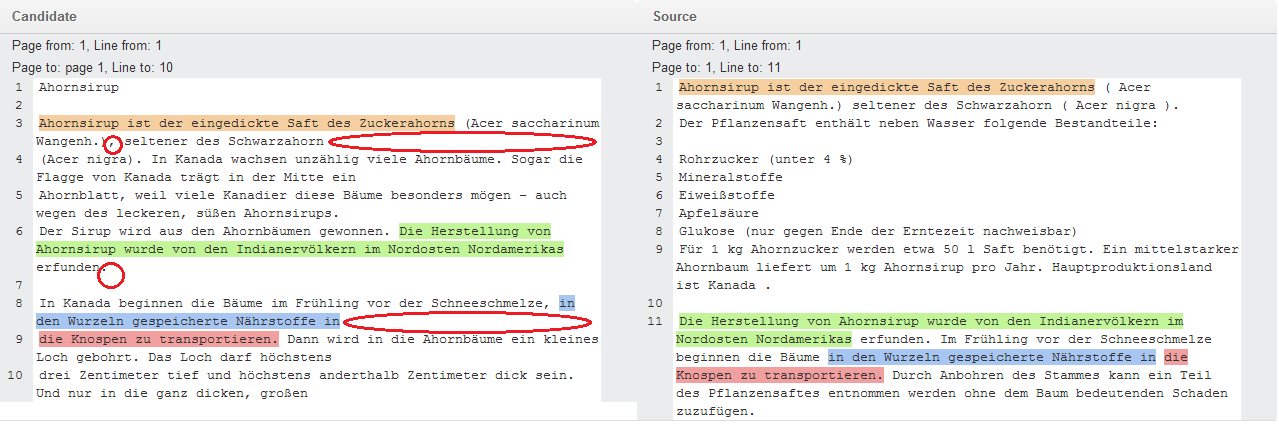
\includegraphics[width=0.97\textwidth]{images/strict_algo.png}
  }
  \caption{a strict comparison algorithm}
  \label{fig:report_deckblatt}
\end{figure}

Here is the source code of compare text function

\begin{lstlisting}
private static function compareText($documents, $min_run_length){
    $documents_len = array();

    $final_match_list = array();
    $match_table = array();
    $docs = sizeof($documents);

    for($doc_idx = 0; $doc_idx < $docs; $doc_idx++){
      $doc = $documents[$doc_idx];
      $tokens = sizeof($doc) - $min_run_length + 1;
      $doc_len = sizeof($doc);
      $documents_len[$doc_idx] = $doc_len;

      // If the word is smaller than the min_run_length, do not analyse it
      if($tokens <= 0){
        continue;
      }

      $min_token_idx = 0;

      for($token_idx = 0; $token_idx < $tokens; $token_idx++){
        $match = array_slice($doc, $token_idx, $min_run_length);
        $match_loc = array($doc_idx, $token_idx);
        $match_tag = implode(" ", $match);

        if(array_key_exists($match_tag, $match_table)){
          if($token_idx >= $min_token_idx){
            $best_match = array($doc_idx, $token_idx, -1, 0, 0);
            $matches = $match_table[$match_tag];
            $nr_matches = sizeof($matches);
            for($idx = 0; $idx < $nr_matches; $idx++){
              $match_peer = $matches[$idx];
              $peer_doc_idx = $match_peer[0];
              $peer_doc = $documents[$peer_doc_idx];
              $peer_token_idx = $match_peer[1] + $min_run_length;
              $peer_len = $documents_len[$peer_doc_idx];
              $our_token_idx = $token_idx + $min_run_length;

              if($peer_doc_idx == $doc_idx){
                continue;
              }

              while($peer_token_idx < $peer_len
              && $our_token_idx < $doc_len
              && $peer_doc[$peer_token_idx] == $doc[$our_token_idx]){
                $peer_token_idx++;
                $our_token_idx++;
              }

              $len = $our_token_idx - $token_idx;
              if($len > $best_match[4]){
                $best_match[2] = $match_peer[0];
                $best_match[3] = $match_peer[1];
                $best_match[4] = $len;
              }
            }

            if($best_match[2] != -1){
              array_push($final_match_list, $best_match);
              $min_token_idx = $token_idx + $best_match[4];
            }
          }
          array_push($match_table[$match_tag], $match_loc);
        }else{
          $match_table[$match_tag] = array($match_loc);
        }
      }
    }
    return $final_match_list;
  }
\end{lstlisting}

\subsubsection{Applying the color to the matched texts}

For marking the color to the matched text passages in plagiarized and source documents, we used the HTML \textit{<span>}-tag to define in which text passage the color will be applied. The \textit{<span>}-tag had a class-attribute named \textit{fragmark-x} with \textit{x} from \textit{1-9} performing one of nine different colors. The CSS color attributes will applied to the text passage corresponding to the class name.

This is the function to apply color to the text passage.

\begin{lstlisting}
private static function getMarkedTexts($comparedTexts, $wordsLeft, $wordsRight, &$listLeft, &$listRight){
    // Colors have css classes "fragmark1" to "fragmark9"
    $col = 0;
    $nr_col = 9;
    
    for($i = 0; $i < sizeof($comparedTexts); $i++){
      $res = $comparedTexts[$i];
      $wordsLeft[$res[3]] = "<span class=\"fragmark-$col\">" . $wordsLeft[$res[3]];
      $wordsLeft[$res[3] + $res[4] - 1] = $wordsLeft[$res[3] + $res[4] - 1] . "</span>";

      $wordsRight[$res[1]] = "<span class=\"fragmark-$col\">" . $wordsRight[$res[1]];
      $wordsRight[$res[1] + $res[4] - 1] = $wordsRight[$res[1] + $res[4] - 1] . "</span>";

      $col = ($col + 1) % $nr_col;
    }
    
    // At this point the text is exploded word by word, now the line breaks have to be added again, as in the original document
    $resultLeft = Unplagged_CompareText::addLinebreaks($listLeft, $wordsLeft);
    $resultRight = Unplagged_CompareText::addLinebreaks($listRight, $wordsRight);

    return array("left"=>$resultLeft, "right"=>$resultRight);
  }
\end{lstlisting}

And the CSS attributes

\begin{lstlisting}
/*colours for the simtext operation (compare function) to mark the same texts*/
.fragmark-0 { background-color: #f5cf9f; }
.fragmark-1 { background-color: #c2f598; }
.fragmark-2 { background-color: #a7c6f2; }
.fragmark-3 { background-color: #f29f9f; }
.fragmark-4 { background-color: #aff2be; }
.fragmark-5 { background-color: #e8a3ff; }
.fragmark-6 { background-color: #e6e181; }
.fragmark-7 { background-color: #b8b8ff; }
.fragmark-8 { background-color: #f5cf9f; }
.fragmark-9 { background-color: #a5e6ed; }
\end{lstlisting}

\subsection{Uses of text comparison function in Unplagged}
The function text comparison was an important feature which was used much in many different sections in our workbench.

\subsubsection{Fragment modify form}

In fragment modify form the user could create a new fragment. In addition he could see the compared text passage with colors directly while adjusting the form as well. This feature was enabled by using an ajax function combining with an onchange-event in Javascript.

\begin{figure}[!h]
  \centering
  \fbox{
    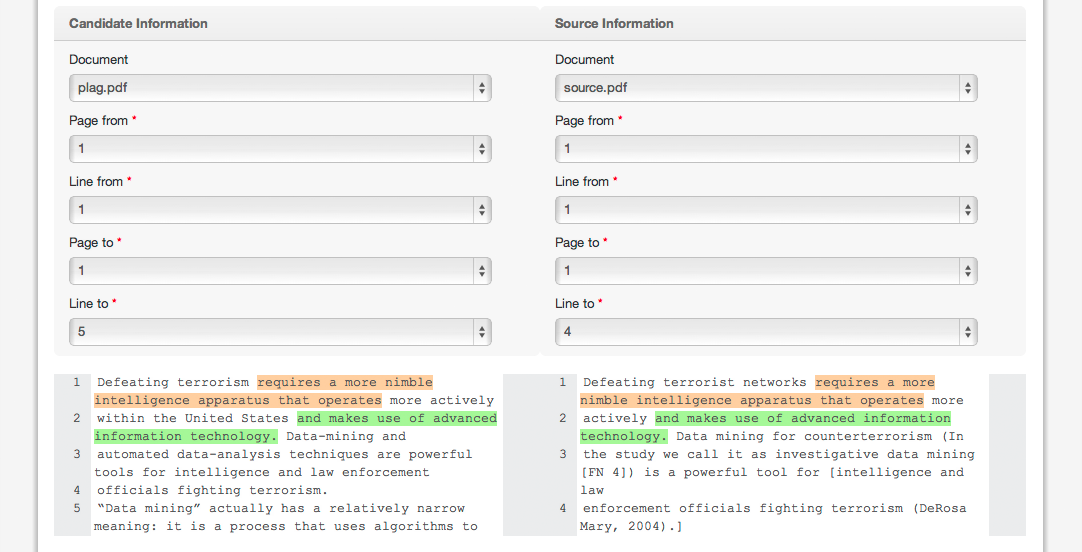
\includegraphics[width=0.97\textwidth]{images/fragment-form.png}
  }
  \caption{Text comparison function in fragment modify form}
  \label{fig:report_deckblatt}
\end{figure}

Here is the code in Jquery

\begin{lstlisting}[caption=Cropping an image to a square aspect ratio]
// executes a simtext comparison in fragment modify form
  function compareTexts() {
    if($("#candidateLineFrom").length != 0) {
      $.post("/document_page/compare", {
        candidateLineFrom: $("#candidateLineFrom").val(),
        candidateLineTo: $("#candidateLineTo").val(),
        sourceLineFrom: $("#sourceLineFrom").val(),
        sourceLineTo: $("#sourceLineTo").val(),
        highlight: true
      }, function(response) {
        if($('#candidateText').length == 0) {
          $('#fieldset-candidateGroup').append('<div id="candidateText" class="src-wrapper"/>');
          $('#fieldset-sourceGroup').append('<div id="sourceText" class="src-wrapper"/>');
        }
        $('#candidateText').html(response.data.plag);
        $('#sourceText').html(response.data.source);
      }, "json");
    }
    return false;
  }
  $("#candidateLineFrom, #candidateLineTo, #sourceLineFrom, #sourceLineTo").change(function(){
    compareTexts();
  });
  compareTexts();
\end{lstlisting}

\subsubsection{Fragment show view }

After a new fragment was created, the user could see it in details by clicking on the link of the fragment. The fragment view page shows on the left side the plagiarized text, and on the right side the source. There was also a button to hide/show the colors. If the user hit the button ''Hide color'' the text would be shown with no colors.

There might be a small improvement in comparison with Vroniplag, that the page and the lines of the fragment would be shown here not manually, but automatized.

\begin{figure}[!h]
  \centering
  \fbox{
    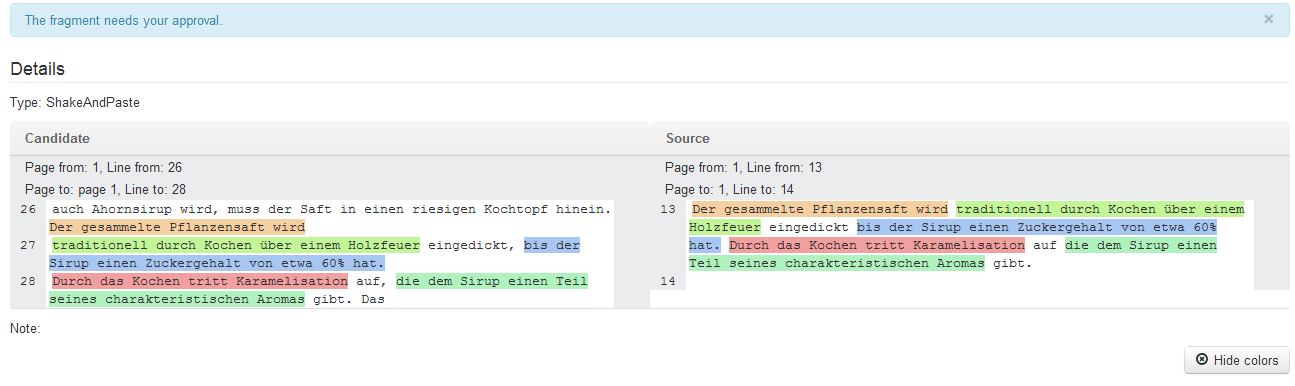
\includegraphics[width=0.97\textwidth]{images/frag_view.png}
  }
  \caption{Text comparison function in fragment show view with colorsr}
  \label{fig:cropping-avatar}
\end{figure}

\begin{figure}[!h]
  \centering
  \fbox{
    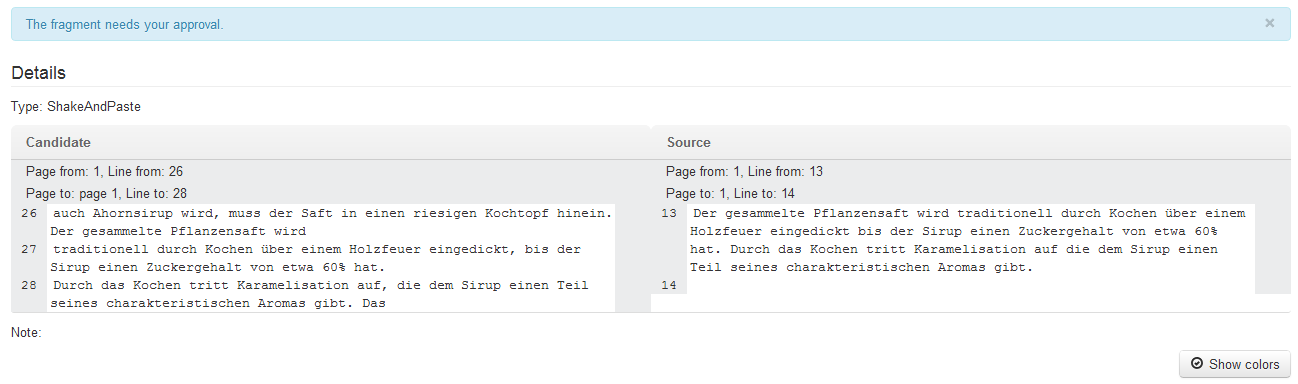
\includegraphics[width=0.97\textwidth]{images/frag_view_plain.png}
  }
  \caption{Text comparison function in fragment show view with no colorsr}
  \label{fig:cropping-avatar}
\end{figure}

\subsubsection{Compare a document with all possible sources from database}

The text compare function could be used to compare a document with many other documents from Unplagged's database. This process could take a lot of time because it depended on the document's size and the number of the sources which the document would be compared with.
We used a cron job to control when the process was finished. After that the created report could be opened.

The report was an HTML text and could be seen directly on the browser.

\begin{figure}[!h]
  \centering
  \fbox{
    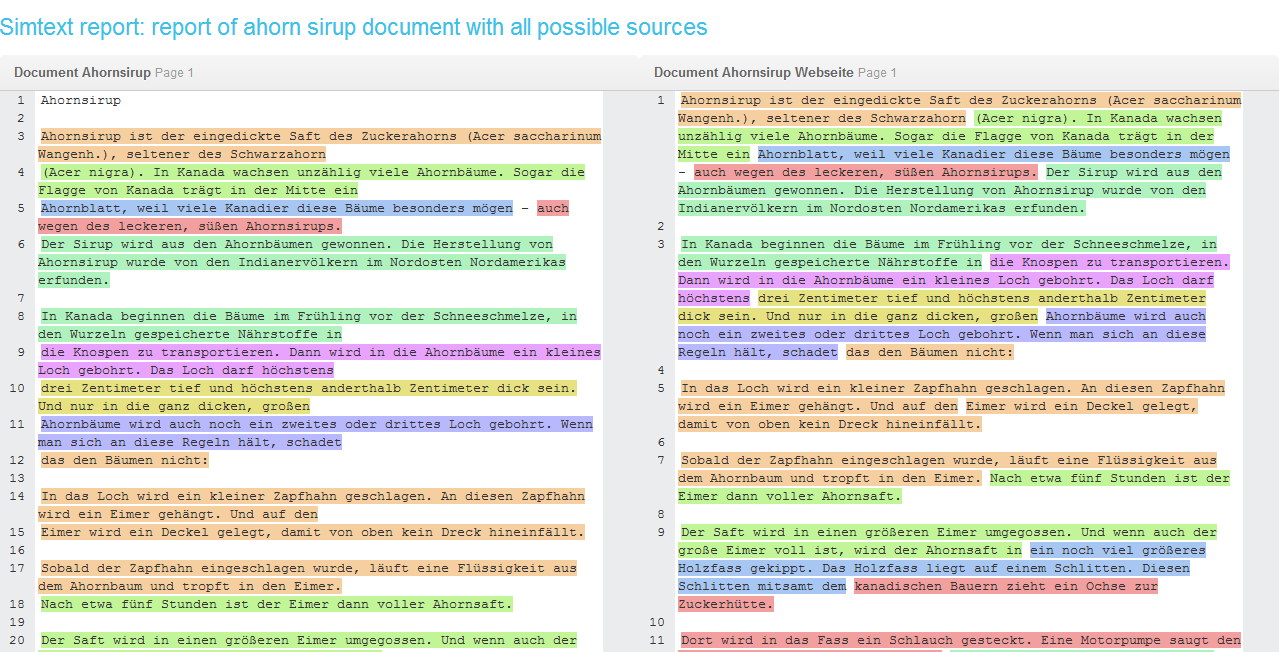
\includegraphics[width=0.97\textwidth]{images/sim_report_1.png}
  }
\fbox{
      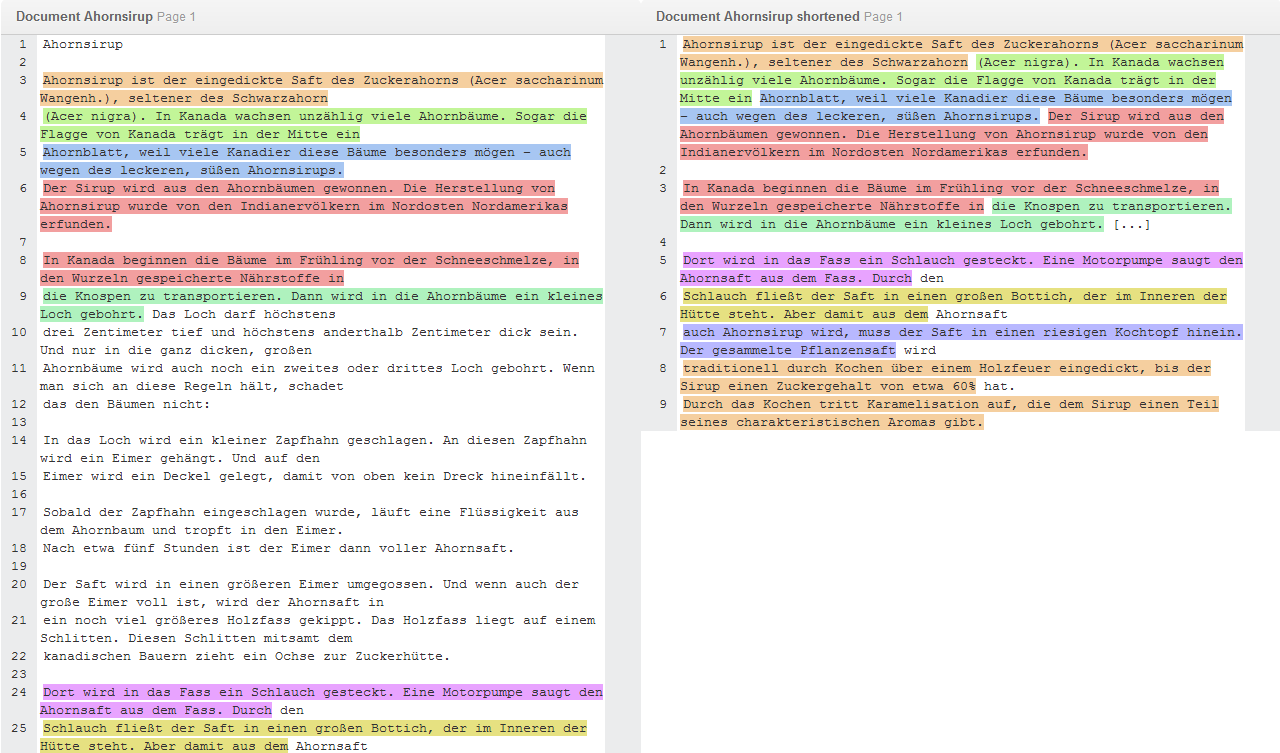
\includegraphics[width=0.97\textwidth]{images/sim_report_2.png}
  }
  \caption{Simtext of many documents}
  \label{fig:Simtext of many documents}
\end{figure}

\pagebreak

\section{Bibtex Metadata}

Bibtex function was another feature in our workbench. Based on VroniPlag, Bibtex was created to provide the user an overview of the document's bibliographic information. The user had the possibility to add the bibtex information of a document through the document modify form when he created a new document. 

In the document modify form there was an extra section for bibtex information. In this section, the bibtex modify form was first shown in its full form. There were over 20 fields in it. All of fields were taken from VroniPlag. The fields \textit{Author} and \textit{Title} must be filled, the field \textit{Year} could be filled as \textit{o.J (ohne Jahrgang)} if it was unknown.

\begin{figure}[!h]
  \centering
  \fbox{
    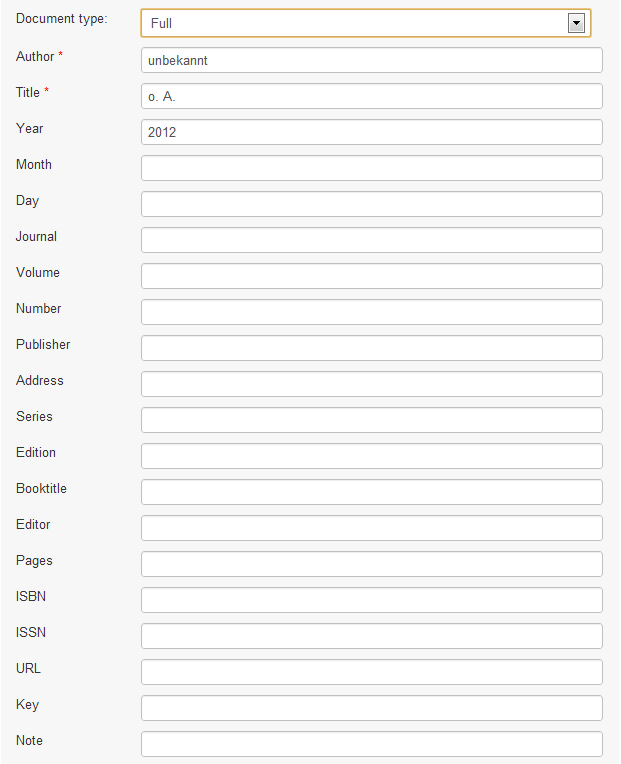
\includegraphics[width=0.97\textwidth]{images/bib_full.png}
  }
  \caption{Bibtex full form}
  \label{fig:Bibtex_full_form}
\end{figure}

If the user wanted to specify a type for his document, there were also 3 separated subforms available:

\begin{itemize}
\item book
\item periodical
\item essay
\end{itemize}

\begin{figure}[!h]
  \centering
  \fbox{
    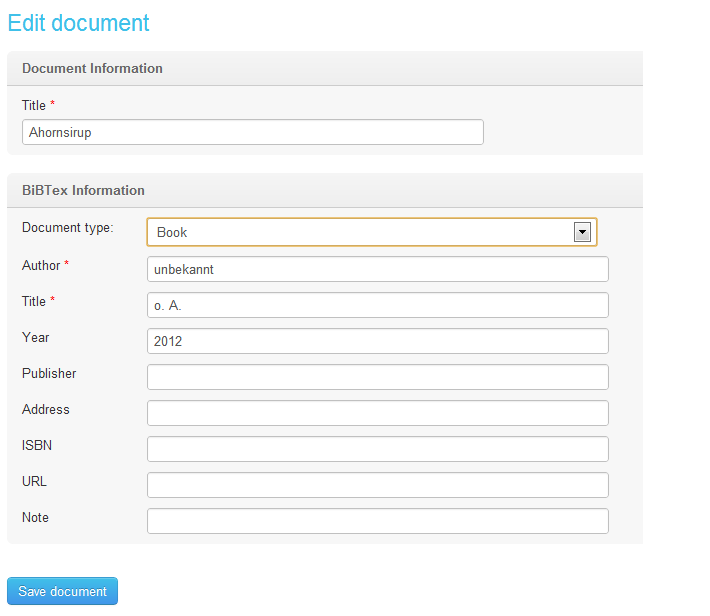
\includegraphics[width=0.97\textwidth]{images/bib_book.png}
  }
  \caption{Bibtex book form}
  \label{fig:Bibtex_book_form}
\end{figure}

\begin{figure}[!h]
  \centering
  \fbox{
    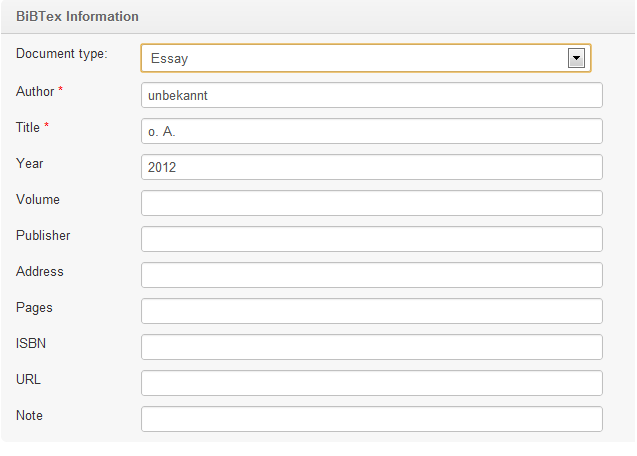
\includegraphics[width=0.97\textwidth]{images/bib_essay.png}
  }
  \caption{Bibtex essay form}
  \label{fig:Bibtex_essay_form}
\end{figure}

\begin{figure}[!h]
  \centering
  \fbox{
    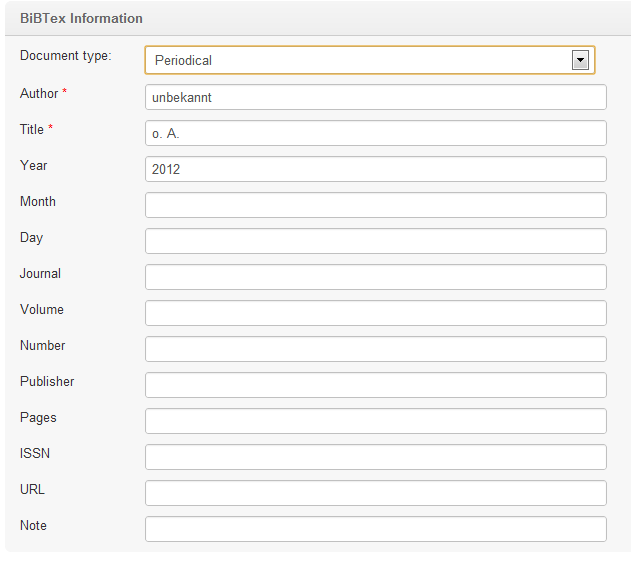
\includegraphics[width=0.97\textwidth]{images/bib_periodical.png}
  }
  \caption{Bibtex periodical form}
  \label{fig:Bibtex_periodical_form}
\end{figure}

After saving bibtex information, the user could see it again by the tab Bibliography in Unplagged. By Bibliography, there was a list of all the documents with their bibtex information are shown. If the user would like to change something, he could choose the action button to come back to the document modify form.

\begin{figure}[!h]
  \centering
  \fbox{
    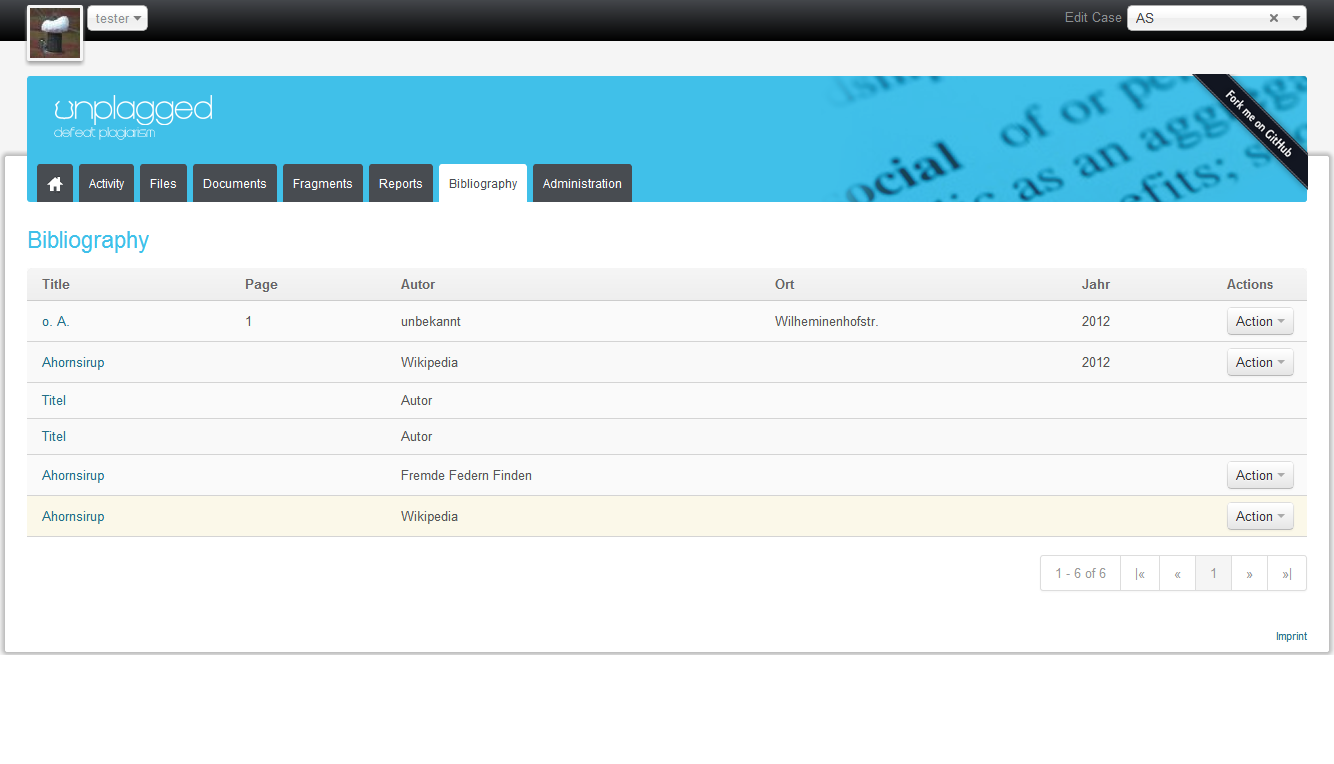
\includegraphics[width=0.97\textwidth]{images/bib_list.png}
  }
  \caption{Bibliography list}
  \label{fig:Bibliography_list}
\end{figure}

If the user clicked on a bibtex link, he would see the details of the bibtex information of the document. More especially, to give the user an overview, that which fragments had belonged to this bibtex, a list of those fragments with the comparison and colors would also be shown here.

\begin{figure}[!h]
  \centering
  \fbox{
    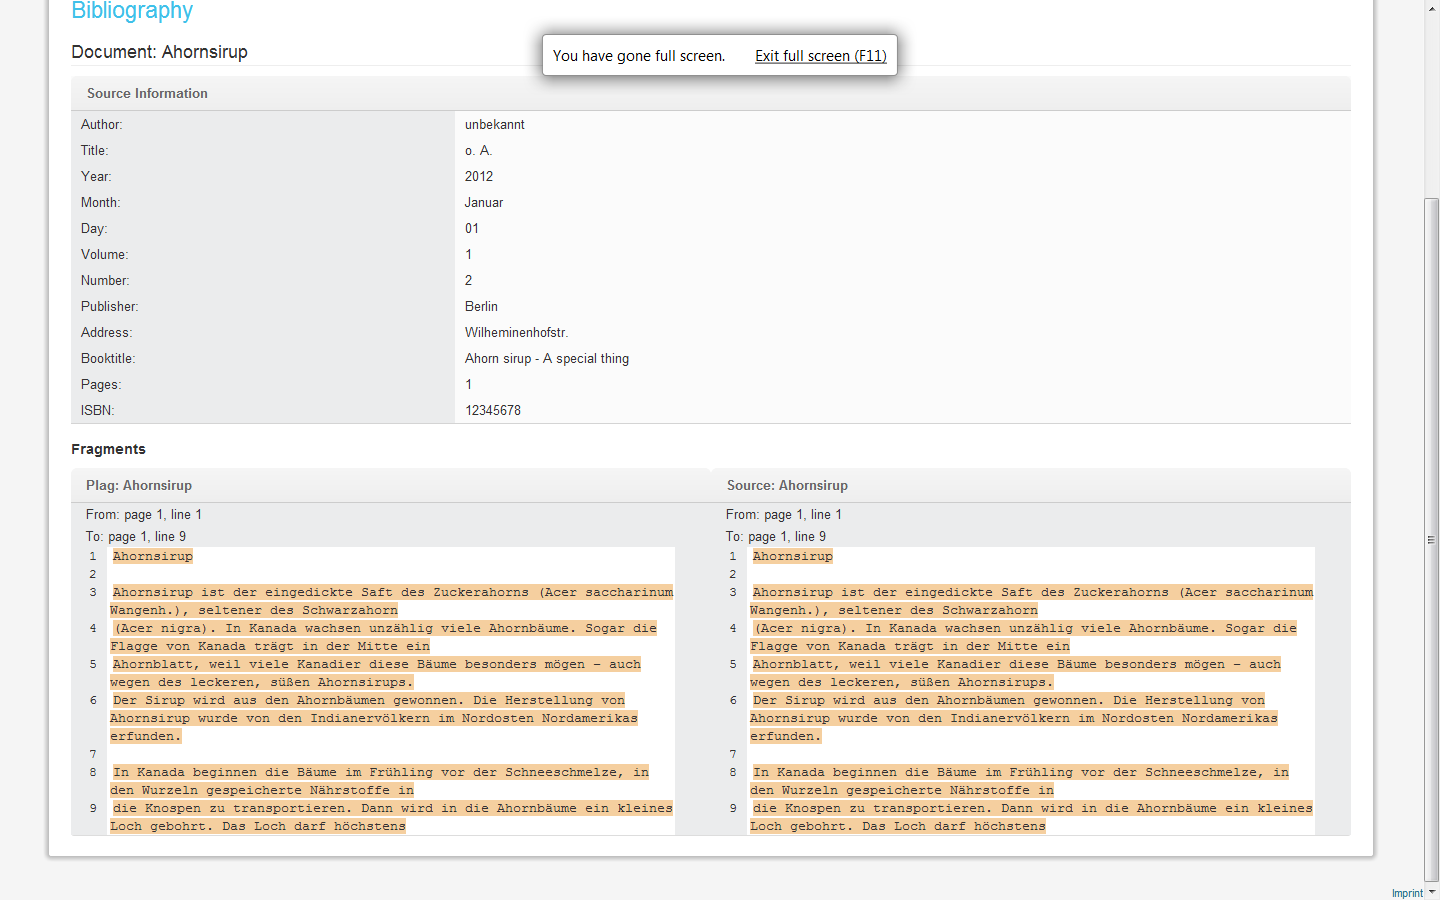
\includegraphics[width=0.97\textwidth]{images/bib_frag_view.png}
  }
  \caption{view of bibtex information with fragments belong to it}
  \label{fig:Bibliography_frag_view}
\end{figure}

\chapter{Showtime}\label{chap:Showtime}

Every semester, students of the "College of Engineering and Economic Berlin" are presenting their bachelor and master projects at a college fair called "Showtime". The event takes place at the end of each semester. Each group has 20 minutes to present their work. On this event professors and visitors have the opportunity to learn about the various projects and groups. At the same time the professors are evaluating the students' work - that is an important part of the course.

Before the "Showtime" started a lot of planning was necessary - from the actual presentation to brochures and posters. Everything needed to be planned and organized.

\section{Presentation}

The main goal of the presentation was bring our software closer to visitors and professors. 
Within the presentation the our software system on one hand was declared and shown, on the other hand substantiate with the help of theoretical foundations.

As a technical basis, we used the online presentation toll calles "impress.js", which enables similar to the Flash presentation tool "Prezi" spatial effects. With impress.js you can create individual slides which are placed in a three-dimensional space. The difference between "Prezi" and "impress.js" is the used technology of "impress.js"- CSS3 and Javascript, so you don´t have to install Adobe Flash. \footnote{http://matthiasschuetz.com/impress-js-effektvolle-zoom-praesentationen-mit-css3 - Date: 24.07.2012}.


\begin{figure}[!h]
  \centering
  \fbox{
    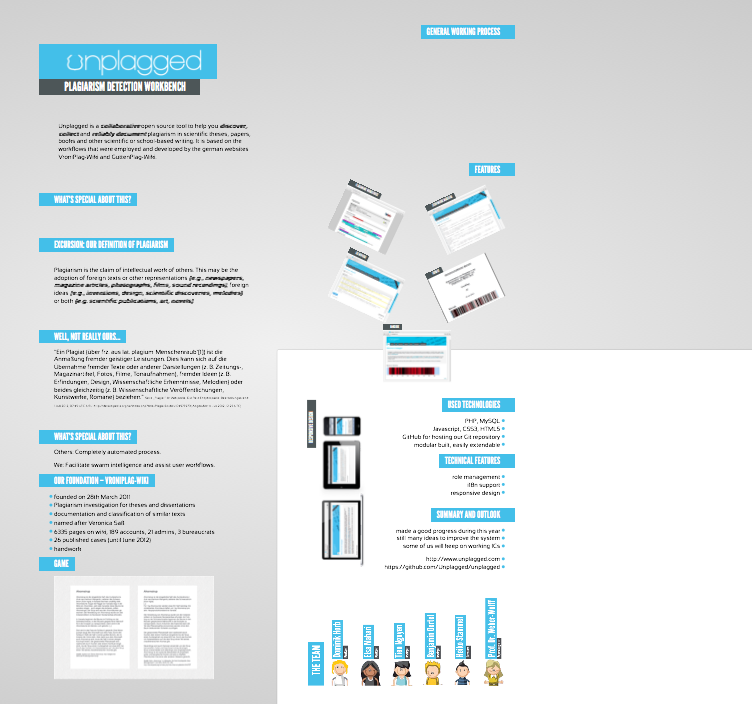
\includegraphics[width=0.97\textwidth]{images/presentation-1.png}
  }
  \caption{Our presentation in impress.js}
  \label{fig:impress.js}
\end{figure}

\subsection{Presentation sequence}
Before the start of our 20 minute presentation, we distributed handouts and pens. These handouts two different texts: On the left the plagiarism candidate to the right the source from Wikipedia.
After we had introduced to ourselves, one of the students led to the presentation. He explained the meaning and purpose of our software and the advantages and differences compared to competitors. Afterwards another group member gave an overview of the history and work of our client "Vroniplag". 
In the third part a group member entered into the handouts, to explain the visitors and professors what it was all about the game. It was about to clarify the difficulties and the effort in the finding process of plagiarism - the daily bread of our professor. For this purpose the visitors had to compare the two texts of the handout and highlight any similarities with the pen. Of course, 50 percent of the text were plagiarized.
Then our six-minute film was shown. The film explains the functionality of our software. 
After the audience had gained a glimpse into the software, another group member explained the features of the software in detail. After this we explained, which technologies were used to create the software. Finally, we ventured a look into the future of "Unplagged", lets say we designed future plans for the software.


\begin{figure}[!h]
  \centering
  \fbox{
    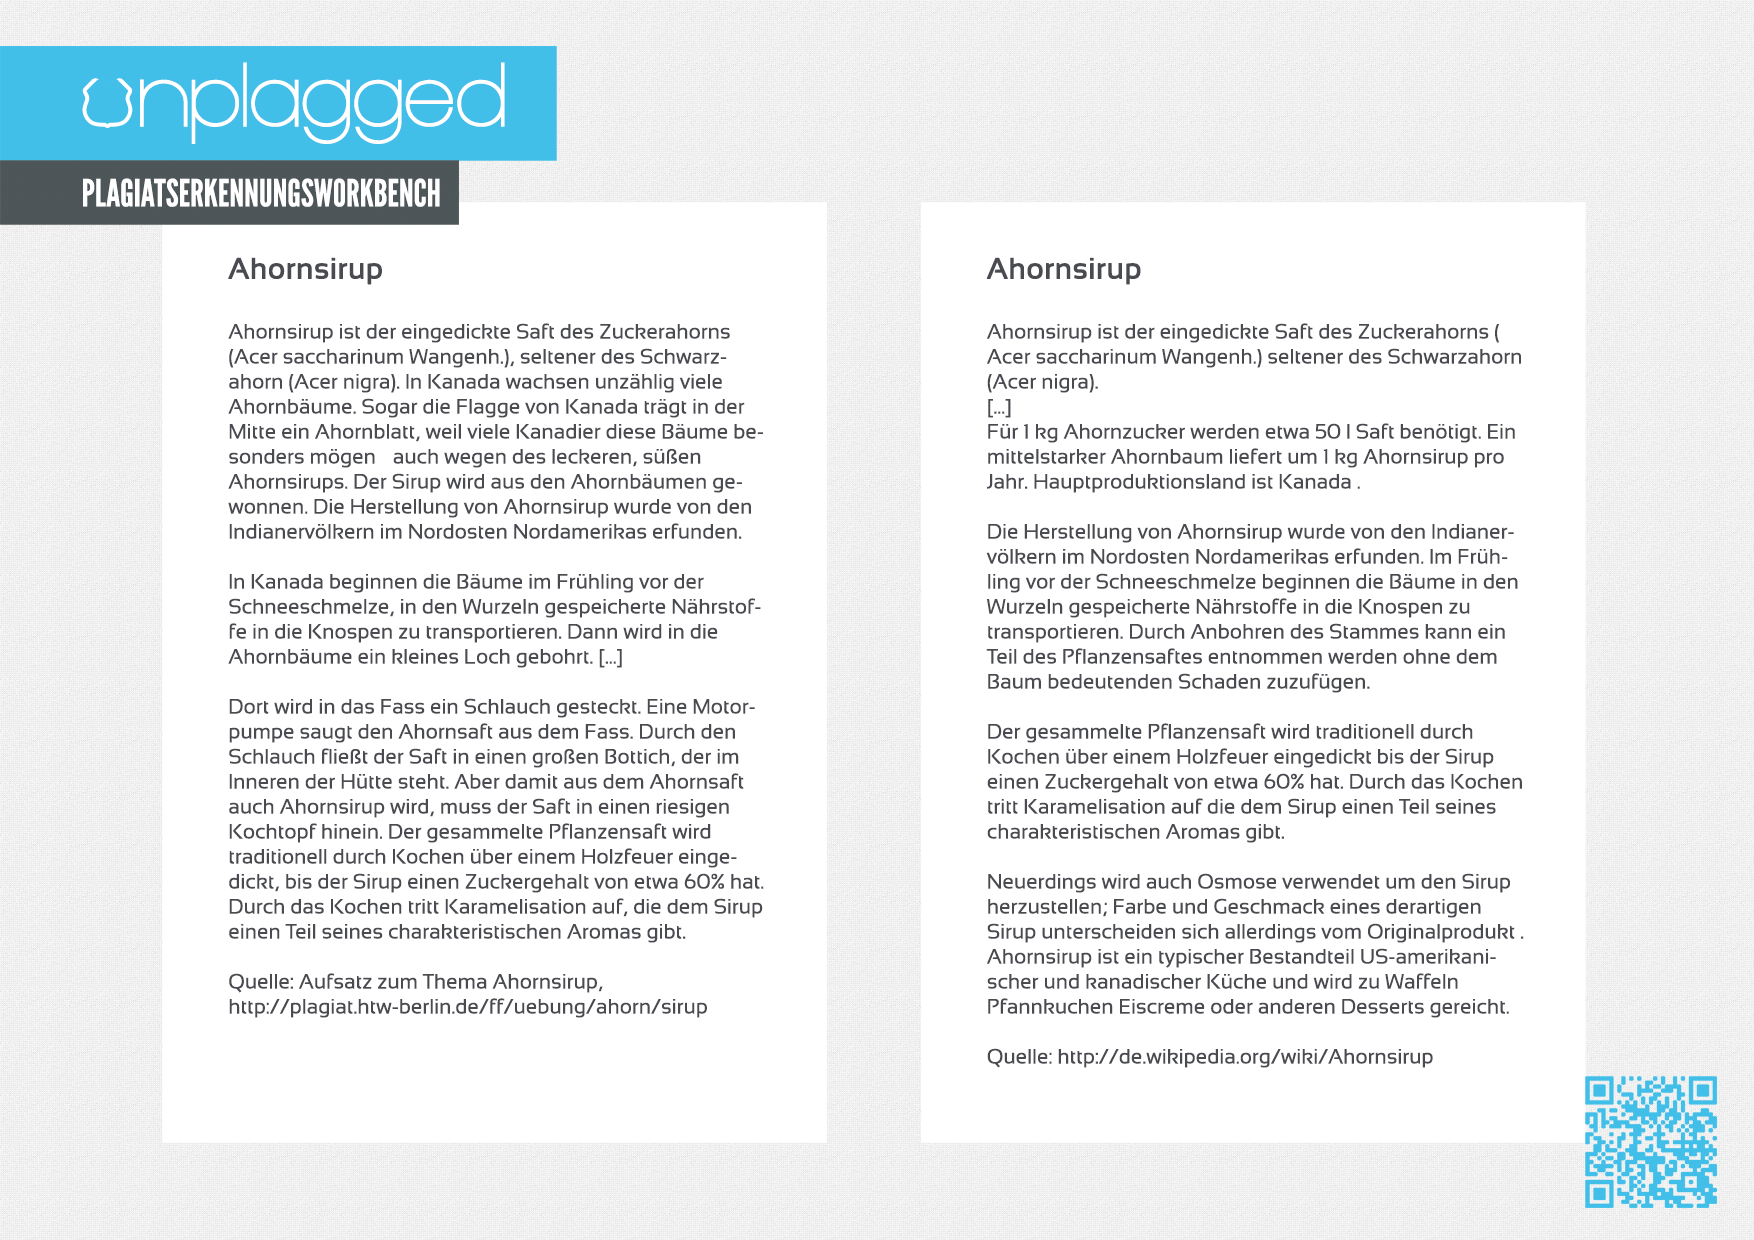
\includegraphics[width=0.97\textwidth]{images/game_handout.png}
  }
  \caption{Game Handout}
  \label{fig:game-handout}
\end{figure}



\subsection{Presentation movie}
The aim of the film was on the one hand to make the software even understandable for laymen, on the other hand to loosen the presentation. The film consisted of animations, which suggested the spectator would himself use the software and analyze a document for plagiarism. Additionally the presentation of the film was shown continuously at the booth.

\begin{figure}[!h]
  \centering
  \fbox{
    
\includegraphics[width=0.5\textwidth]{images/descriptive-headline.png}
  }
  \caption{Movie descriptive headline}
  \label{fig:descriptive-headline}
\end{figure}


\pagebreak 


\subsection{Movie creation}
For film production, we used Adobe After Effects and Adobe Photoshop. The film showed the chronological order of the plagiarism process. This works best for the spectator when he sees the screen, he would also actually see before them. Each new scene was launched with a descriptive headline. After this we used a screencast software to show how to log in, upload documents, searches for plagiarism, divides into fragments, creating documents and automated comparing of documents- in short, how the software works. The mouse cursor was marked for greater clarity in color constantly. Instead of a rigid voice-over, we let a group member to take the voice-over. So we were able to respond optimally to questions of the audience.


\begin{figure}[!hbtp]
  \centering
  \fbox{
    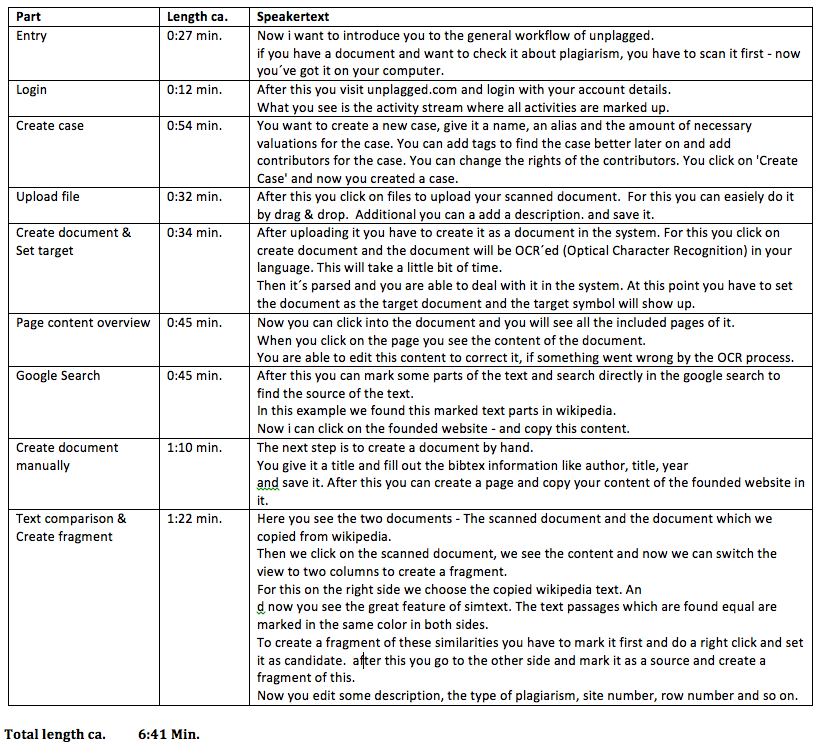
\includegraphics[width=1\textwidth]{images/movie-parts.png}
  }
  \caption{Presentation movie structure}
  \label{fig:fpresentation-movie-structure}
\end{figure}

\begin{figure}[!hbtp]
  \centering
  \fbox{
    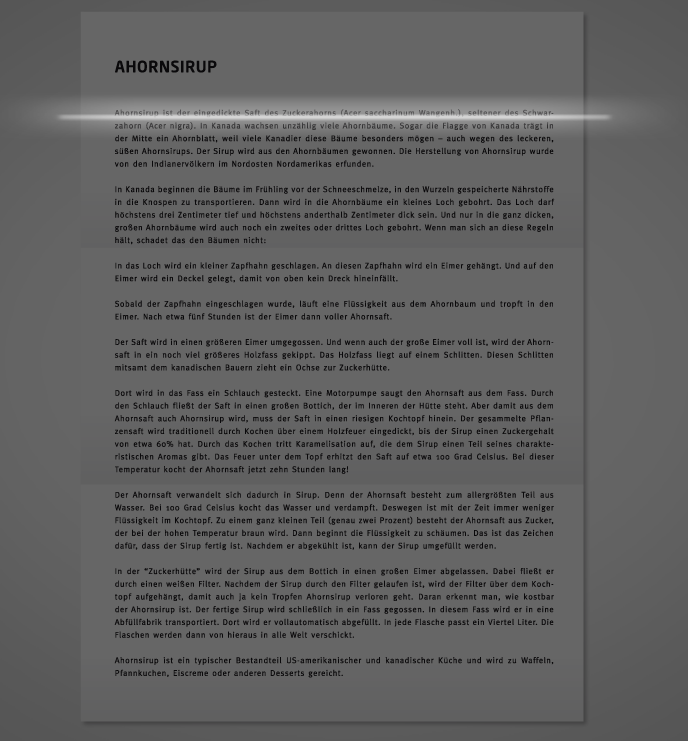
\includegraphics[width=0.5\textwidth]{images/scan-animation.png}
  }
  \caption{Scan Animation}
  \label{fig:scan-animation}
\end{figure}

\begin{figure}[!hbtp]
  \centering
  \fbox{
    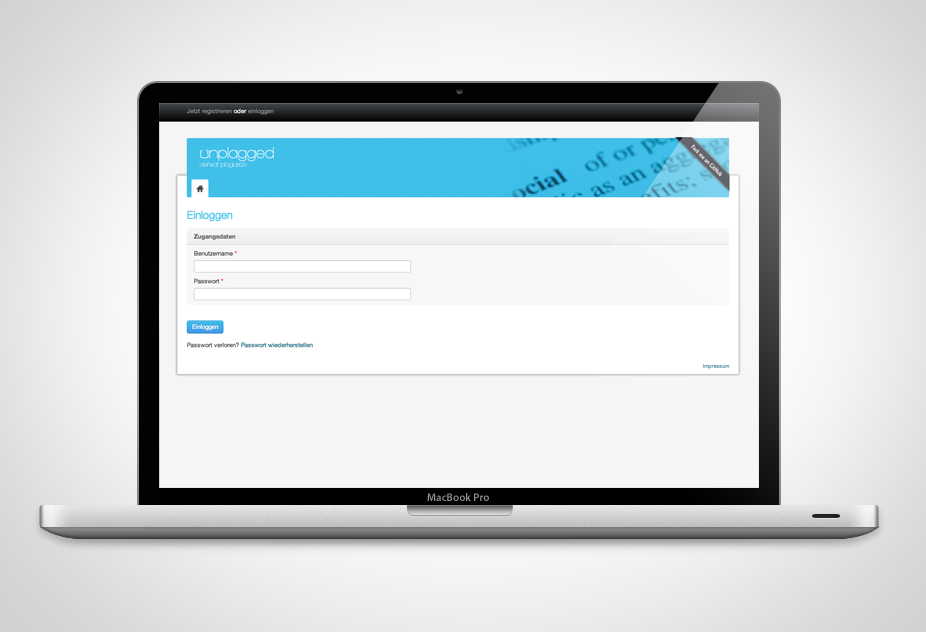
\includegraphics[width=0.5\textwidth]{images/macbook.png}
  }
  \caption{Macbook animation}
  \label{fig:macbook}
\end{figure}

\pagebreak 


\section{Paperwork}
At the beginning it was necessary to make a first concept of the brochure and posters for the unplagged exhibition stand.

\subsection{Brochure}


In addition to various posters, we developed a two-page brochure. The lay out of the booth and could be freely taken by the visitors. It gave a brief outline of our project and the visitors had the opportunity to call back the most important points into memory.
This was the first concept of the brochure, which was kind of a sketch.





\begin{figure}[!hbtp]
  \centering
  \fbox{
    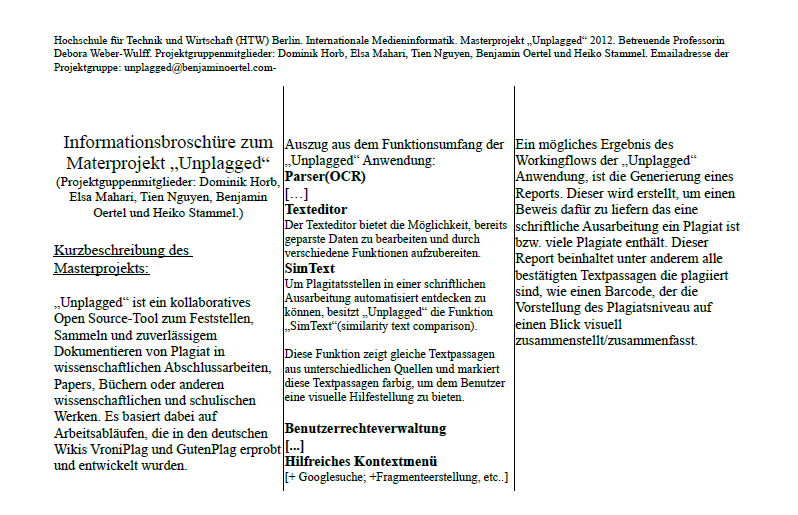
\includegraphics[width=0.97\textwidth]{images/brochure_sketch.png}
  }
  \caption{the first concept of the brochure}
  \label{fig:brochure_sketch}
\end{figure}

Below is the final outlook of the brochure.

\begin{figure}[!hbtp]
  \centering
  \fbox{
    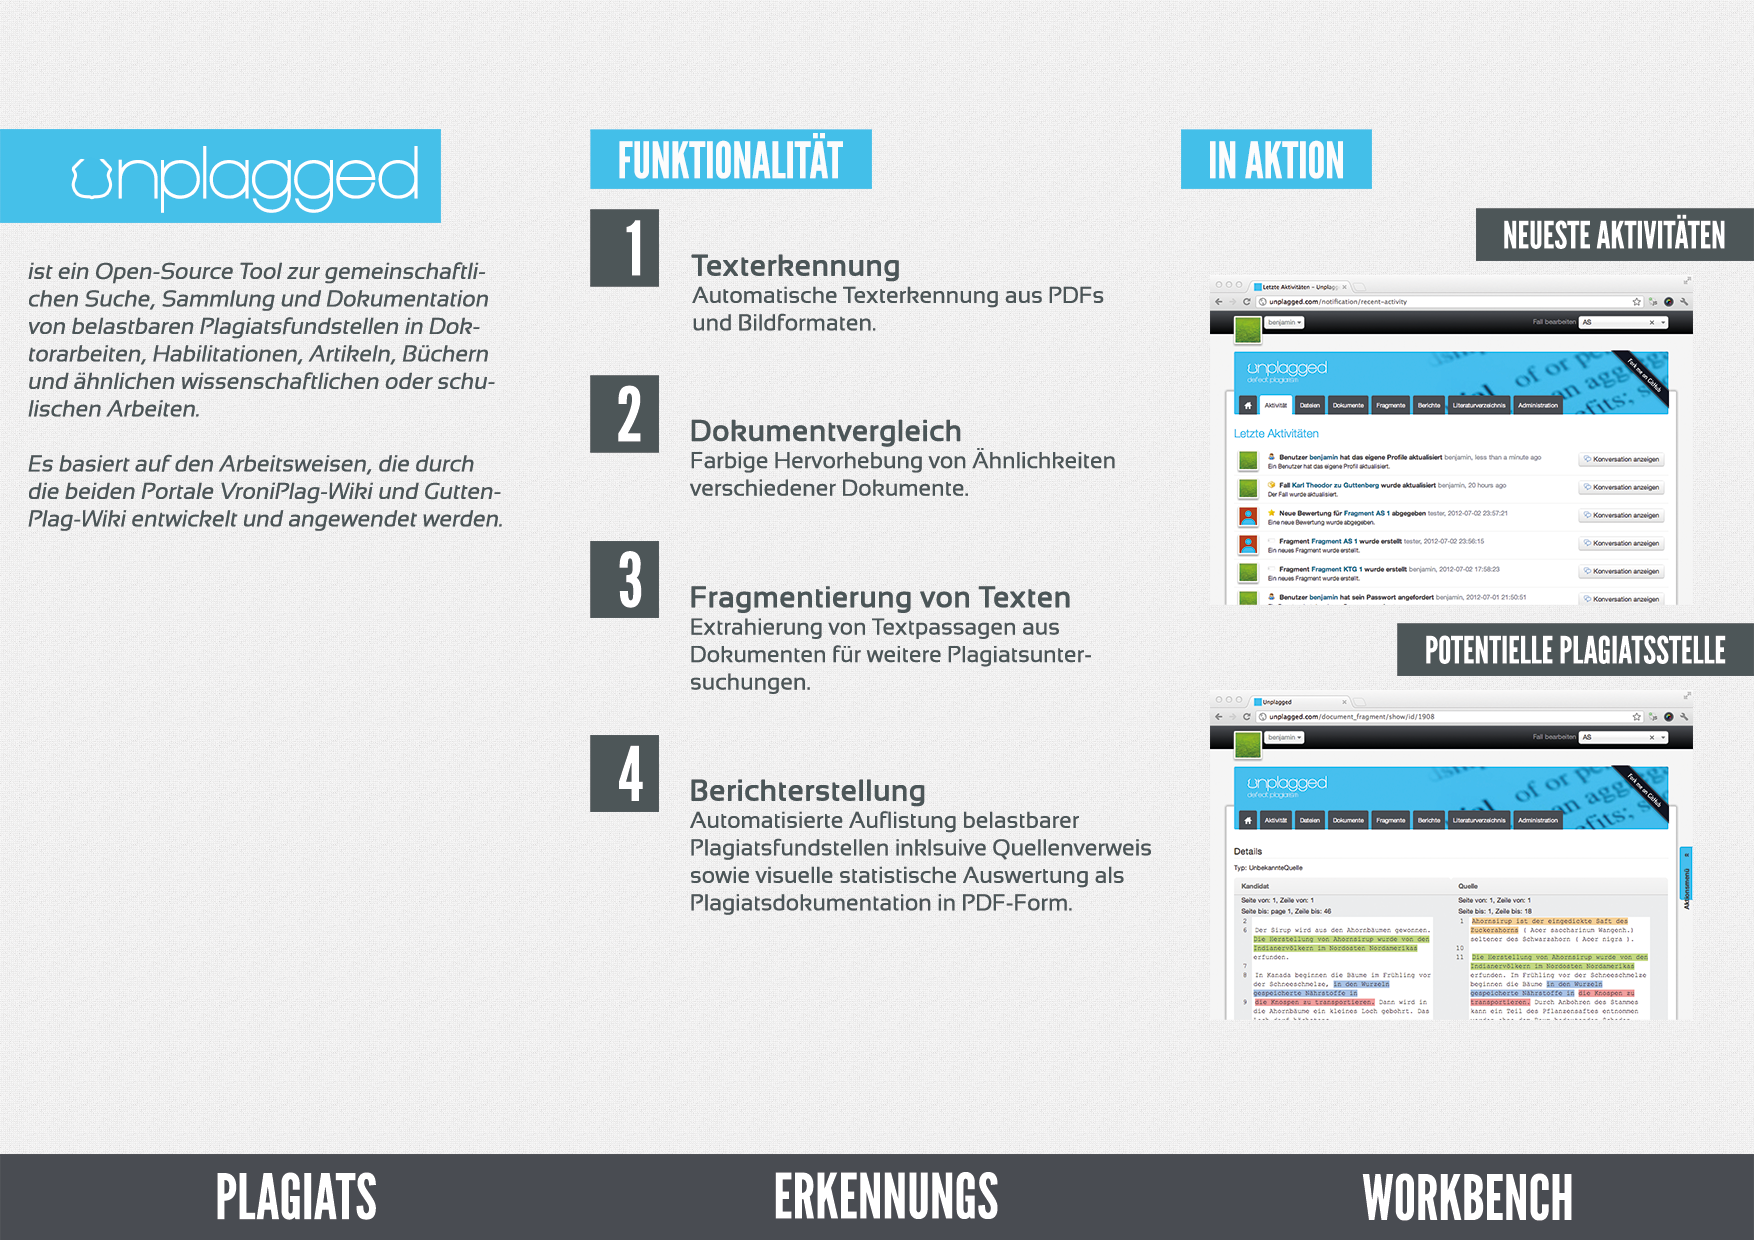
\includegraphics[width=0.97\textwidth]{images/a4_tri-fold_inside.png}
  }
  \caption{the frontside of the final unplagged brochure}
  \label{fig:brochure_final_frontside}
\end{figure}

\begin{figure}[!hbtp]
  \centering
  \fbox{
    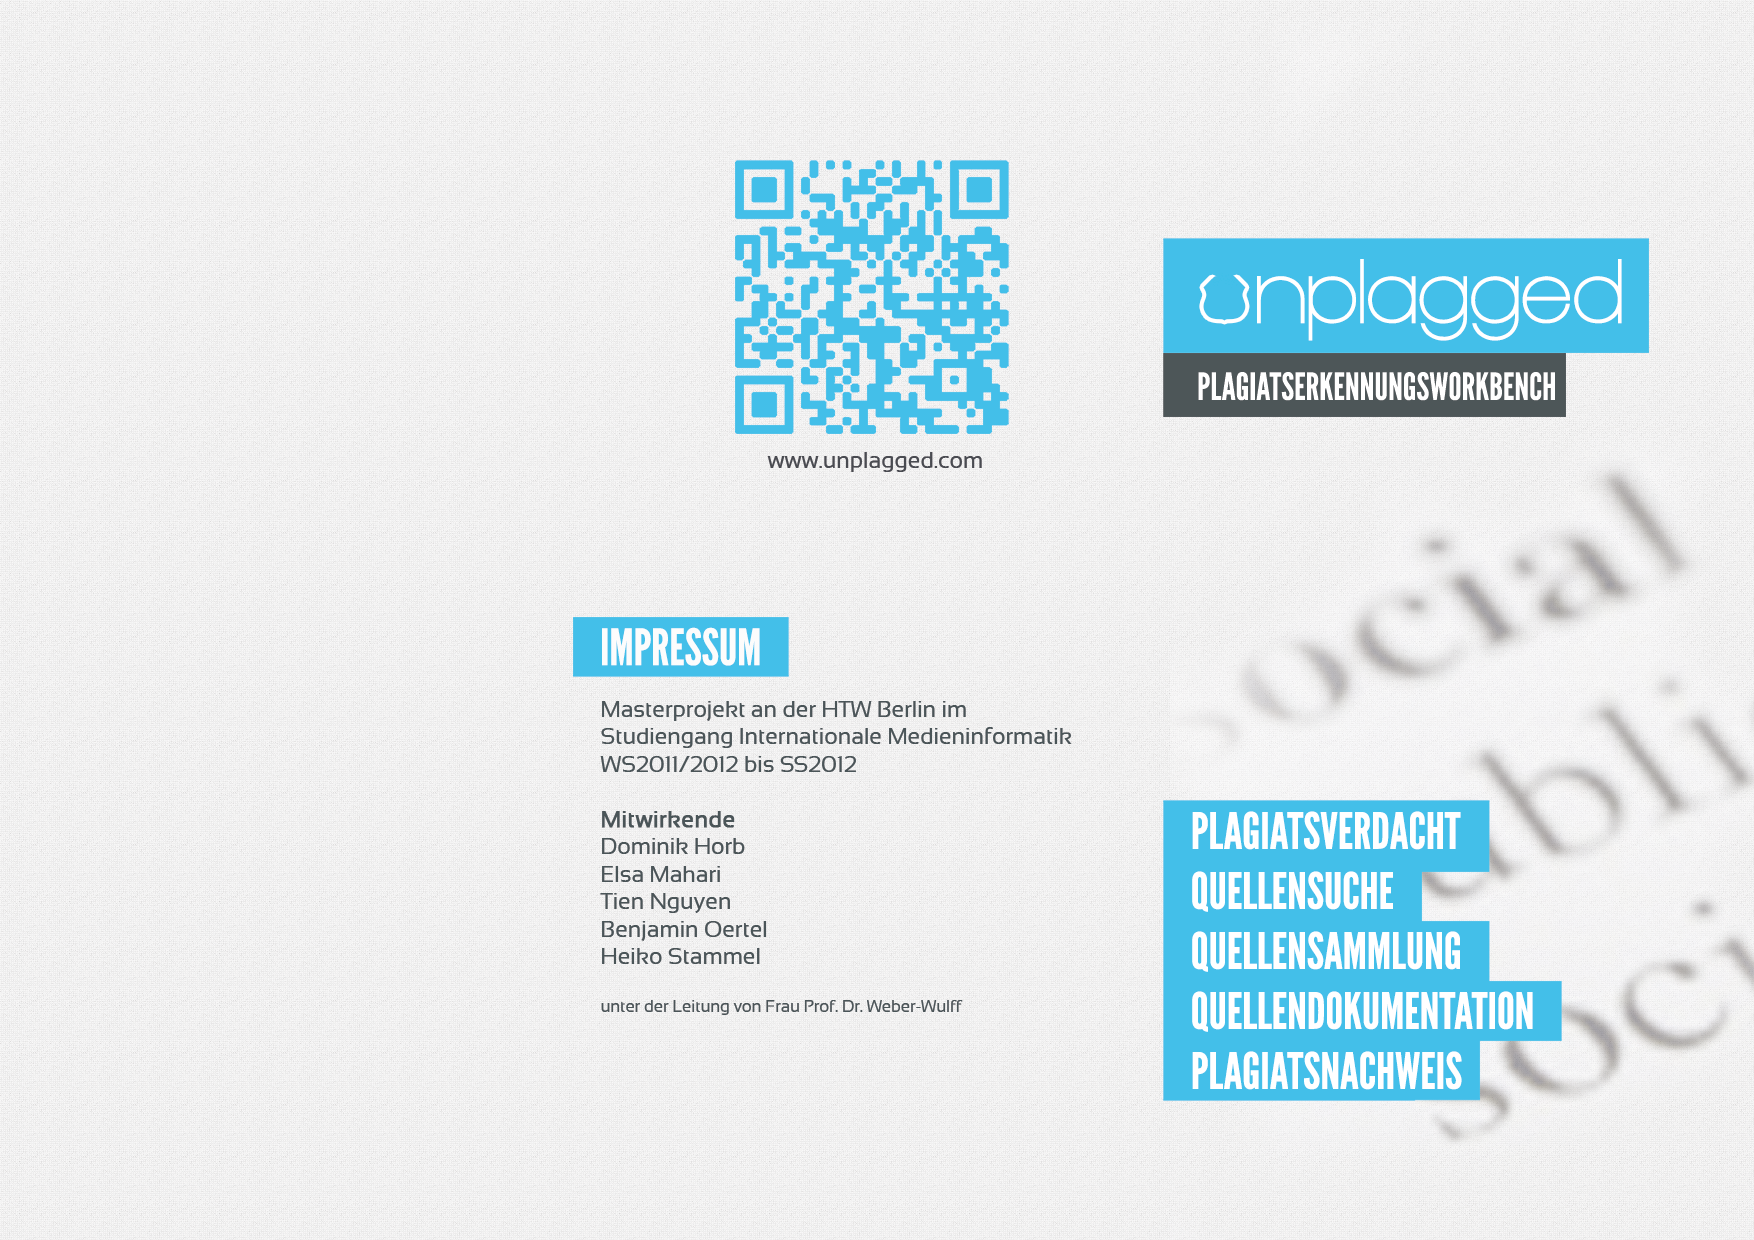
\includegraphics[width=0.97\textwidth]{images/a4_tri-fold_outside.png}
  }
  \caption{the backside of the final unplagged brochure}
  \label{fig:brochure_final_backside}
\end{figure}

\pagebreak 

\subsection{Posters}

The posters were developed mainly for the booth. Visitors and professors could thus provide a first quick overview about our project. At the same time they were supposed to generate attention: 
A technical Poster which gave the visitors an overview about the technology we used, 
a team poster with a survey about the team members, the key features, a programming sprint overview and a poster with the "Unplugged" logo.


\subsubsection{Title Poster}

\begin{figure}[!hbtp]
  \centering
  \fbox{
    \includegraphics[width=0.97\textwidth]{images/a4_logo.png}
  }
  \caption{the title poster}
  \label{fig:poster_title}
\end{figure}

\pagebreak

\subsubsection{Describing Poster}

\begin{figure}[!hbtp]
  \centering
  \fbox{
    \includegraphics[width=0.8\textwidth]{images/a4_poster_general.png}
  }
  \caption{the describing poster}
  \label{fig:poster_describing}
\end{figure}

\pagebreak

\subsubsection{Technical Poster}

Below is a cutout of the technical poster.

\begin{figure}[!hbtp]
  \centering
  \fbox{
    \includegraphics[width=0.8\textwidth]{images/a4_poster_technology.png}
  }
  \caption{the technical poster}
  \label{fig:poster_technical}
\end{figure}

\pagebreak 


\section{Exhibition stand}

The best possible way to present our software was to hang three posters in the background. 



\begin{figure}[!hbtp]
  \centering
  \fbox{
    \includegraphics[width=0.97\textwidth]{images/unplagged_exhibition_stand1.jpg}
  }
  \caption{unplagged exhibition stand}
  \label{fig:unplagged_exhibition_stand1}
\end{figure}

\pagebreak

The stand itself was equipped with three iMacs to be able demonstrate the software.
Once a computer was idle, we let the film run on the desktop.
Additionally, we distributed the brochure with a brief over view About "Unplugged".
The whole day we were about to answer visitors' questions, the offer has been widely used.
Below there are some snapshots of the unplagged exhibition stand.

\begin{figure}[!hbtp]
  \centering
  \fbox{
    \includegraphics[width=0.97\textwidth]{images/DSC_0173.jpg}
  }
  \caption{unplagged exhibition stand}
  \label{fig:unplagged_exhibition_stand2}
\end{figure}

\pagebreak 

\begin{figure}[!hbtp]
  \centering
  \fbox{
    \includegraphics[width=0.97\textwidth]{images/unplagged_exhibition_stand3.jpg}
  }
  \caption{unplagged exhibition stand}
  \label{fig:unplagged_exhibition_stand3}
\end{figure}

\pagebreak

\begin{figure}[!hbtp]
  \centering
  \fbox{
    \includegraphics[width=0.97\textwidth]{images/unplagged_exhibition_stand4.jpg}
  }
  \caption{unplagged exhibition stand}
  \label{fig:unplagged_exhibition_stand4}
\end{figure}

\pagebreak

\begin{figure}[!hbtp]
  \centering
  \fbox{
    \includegraphics[width=0.97\textwidth]{images/DSC_0162.jpg}
  }
  \caption{unplagged exhibition stand}
  \label{fig:unplagged_exhibition_stand4}
\end{figure}

\pagebreak
\chapter{Summary and Outlook}\label{chap:summaryAndOutlook}

During the first project semester, we already immerged into the field of plagiarism detection very deeply. After
we read about exisiting websites and talked to Prof. Dr. Weber-Wulff about her experience and missing features
at VroniPlag, we at least got an idea, how a software system for this domain could look like. After this phase of 
initial research, we 
developed first 
user interface mockups and
a basic layout, before we started the development on some user stories. 

The application of a modified version of Scrum as our agile software development method was a very interesting and new
experience to all of us, but also took us some more time than expected to figure out. But with the use of Redmine for 
keeping track of all 
issues, repository changes and time logs, 
everyone in the team is now able to take a look on the current project state anytime.

All in all, the conditions for a successful development were allocated properly and we already have implemented some 
features of the product backlog, that will be built upon in the next sprints.

Problematic was, that the employed development processes were not as consistent as they should have been. The in 
theory defined rules on how to program and how to test source code properly were not always applied. So one of the 
main goals for the next block of sprints is to improve this proccess. We need to focus on test driven development and 
increase our velocity during the sprints, in order to get stable code more easily. Maybe implementing some kind of 
review process would also help in solving those problems.

Another thing we want to work on is the staging environment we are using. Some features behave differently on Mac 
OS and Windows machines. Since we have only one staging environment, which updates on every commit to our git 
repository, it sometimes happens that a feature working on Windows crashes the staging environment. This is somehow 
nice, because those errors are encountered early, if the preview area is checked properly, but sometimes those problems
can be overlooked. As a solution 
we are thinking about setting up a second pre-staging environment which updates at every commit to the repository 
automatically and 
another more stable server, which can be updated manually via a script as soon as the pre-staging environment is tested properly. 

Even though we wrote down some information about the development process inside the Wiki of Redmine, most of the 
documentation as 
represented in this document had to be 
done in the end of the semester and not continuously during the process. 
In the next semester we are planning to extend and keep the manual up to date at every sprint, which means preferably 
more time for development and less time for documentation in the end.

We hope that this document was helpful to you! Please contact us if you have any questions or remarks.

\large 
\textbf{Best regards, \\
The Unplagged Team}
\begin{appendix}

\chapter{Meetings}\label{ch:Meetings}
The following tables show the minutes of most of the team meetings.

\begin{figure}[htbp]
  \centering
    \includegraphics[width=\textwidth]{images/a_meetings/meeting_6}
  \caption{Meeting minutes no. 6}
  \label{fig:meeting minutes no. 6}
\end{figure}

\begin{figure}[htbp]
  \centering
    \includegraphics[width=\textwidth]{images/a_meetings/meeting_8}
  \caption{Meeting minutes no. 8}
  \label{fig:meeting minutes no. 8}
\end{figure}

\begin{figure}[htbp]
  \centering
    \includegraphics[width=\textwidth]{images/a_meetings/meeting_10}
  \caption{Meeting minutes no. 10}
  \label{fig:meeting minutes no. 10}
\end{figure}

\begin{figure}[htbp]
  \centering
    \includegraphics[width=\textwidth]{images/a_meetings/meeting_11}
  \caption{Meeting minutes no. 11}
  \label{fig:meeting minutes no. 11}
\end{figure}

\begin{figure}[htbp]
  \centering
    \includegraphics[width=\textwidth]{images/a_meetings/meeting_12}
  \caption{Meeting minutes no. 12}
  \label{fig:meeting minutes no. 12}
\end{figure}

\begin{figure}[htbp]
  \centering
    \includegraphics[width=\textwidth]{images/a_meetings/meeting_13}
  \caption{Meeting minutes no. 13}
  \label{fig:meeting minutes no. 13}
\end{figure}

\begin{figure}[htbp]
  \centering
    \includegraphics[width=\textwidth]{images/a_meetings/meeting_15}
  \caption{Meeting minutes no. 15}
  \label{fig:meeting minutes no. 15}
\end{figure}

\begin{figure}[htbp]
  \centering
    \includegraphics[width=\textwidth]{images/a_meetings/meeting_17}
  \caption{Meeting minutes no. 17}
  \label{fig:Meeting minutes no. 17}
\end{figure}

\begin{figure}[htbp]
  \centering
    \includegraphics[width=\textwidth]{images/a_meetings/meeting_18}
  \caption{Meeting minutes no. 18}
  \label{fig:Meeting minutes no. 18}
\end{figure}

\begin{figure}[htbp]
  \centering
    \includegraphics[width=\textwidth]{images/a_meetings/meeting_19}
  \caption{Meeting minutes no. 19}
  \label{fig:Meeting minutes no. 19}
\end{figure}

\chapter{Logged Time As Of March 22, 2012}

The following tables are some example reports generated from the logged time in Redmine. To find the most recent version
of these reports or to generate custom data analysis you can use the \enquote{Report} tool found in Redmine on the \enquote{Overview}
page.

% should be updated later on, now simply to make sure it works
% generate various reports in redmine and export as csv
% don't forget to escape special characters like _ or # in the input .csv, e. g. \_ or \#

\DTLloaddb{overview}{data/timelog-overview.csv}
\begin{table}[htbp]
  \caption{Overview By Member and Month}
  \centering
  \DTLdisplaydb{overview}
\end{table}

\begin{landscape}

\DTLsetseparator{,}

\DTLloaddb{issueMember}{data/timelog-issue-member.csv}
  \centering
 \DTLdisplaylongdb[caption=Overview By Member and Issue]{issueMember}

\DTLloaddb{sprints}{data/timelog-sprints.csv}
\begin{table}[htbp]
  \caption{Overview By Sprints}
  \centering
  \DTLdisplaydb{sprints}
\end{table}

\end{landscape}

\chapter{Mockups}\label{appendix:mockups}

\section{Hand-Drawn}

\begin{figure}[!h]
  \centering
    \includegraphics[width=\textwidth]{mockups/m_compare_result.jpg}
  \caption{Mockup – Compare results – digitalized }
  \label{fig:mCompareResultsMockup}
\end{figure}

\begin{figure}[!h]
  \centering
    \includegraphics[width=\textwidth]{mockups/m_media_list.jpg}
  \caption{Mockup – Media list – digitalized }
  \label{fig:mMediaListMockup}
\end{figure}

\begin{figure}[!h]
  \centering
    \includegraphics[width=\textwidth]{mockups/m_new_case.jpg}
  \caption{Mockup – New case – digitalized }
  \label{fig:1newCaseMockup}
\end{figure}

\begin{figure}[!h]
  \centering
    \includegraphics[width=\textwidth]{mockups/m_new_fragment.jpg}
  \caption{Mockup – New fragment – digitalized }
  \label{fig:1newCaseMockup}
\end{figure}

\begin{figure}[!h]
  \centering
    \includegraphics[width=\textwidth]{mockups/m_new_project.jpg}
  \caption{Mockup – New project – digitalized }
  \label{fig:mNewProjectMockup}
\end{figure}

\clearpage
\section{Digitalized}

\begin{figure}[htbp]
  \centering
    \includegraphics[width=0.86\textwidth]{mockups/1_new_case.png}
  \caption{Mockup – New case – digitalized }
  \label{fig:1newCaseMockup}
\end{figure}

\begin{figure}[!h]
  \centering
    \includegraphics[width=\textwidth]{mockups/2_list_fragments.png}
  \caption{Mockup – List fragments – digitalized }
  \label{fig:2listFragmentsMockup}
\end{figure}

\begin{figure}[!h]
  \centering
    \includegraphics[width=\textwidth]{mockups/3_new_fragment.png}
  \caption{Mockup – New fragment – digitalized }
  \label{fig:3newFragmentMockup}
\end{figure}

\begin{figure}[!h]
  \centering
    \includegraphics[width=0.97\textwidth]{mockups/4_show_fragment_for_approval.png}
  \caption{Mockup – Show fragment for approval – digitalized }
  \label{fig:4showFragmentForApprovalMockup}
\end{figure}

\begin{figure}[!h]
  \centering
    \includegraphics[width=\textwidth]{mockups/5_new_report.png}
  \caption{Mockup – New report – digitalized }
  \label{fig:5newReportMockup}
\end{figure}

\end{appendix}

\bibliography{biblio}
\end{document}